\documentclass[5p,times,twocolumn]{elsarticle}

\usepackage{amsmath,amssymb,amsfonts}
\usepackage{graphicx}
\usepackage{booktabs}
\usepackage{multirow}
\usepackage{makecell}
\usepackage{array}
\usepackage{subcaption}
\usepackage[ruled,linesnumbered]{algorithm2e}
\usepackage[table]{xcolor}
\usepackage{balance}
\usepackage{hyperref}

\journal{ICT Express}

\begin{document}

\begin{frontmatter}

\title{Lineage-Grounded Evaluation of Cell Coupling and State Representations in Human Midbrain Differentiation}


% \author[kit]{Victor Ikenna Kanu}
% \author[lu]{Willaims Paul Nwadiugwu}
% \author[kit]{Dong-Seong Kim\corref{cor}}
% \cortext[cor]{Corresponding author}
% \affiliation[kdu]{organization={Smart Computing Department, Kyungdong University, Global Campus}, country={South Korea}}
% \affiliation[kit]{organization={Department of IT Convergence Engineering,
%   Kumoh National Institute of Technology}, city={Gumi},
%   country={South Korea}}



\begin{abstract}
Models predicting cellular response to chemical perturbation are routinely
benchmarked against baselines, but the assumptions preceding any model are
rarely tested, and a benchmark conducted afterwards cannot distinguish a poor
model from an unsupported premise. This work evaluates four such assumptions
under a protocol in which every statistic and threshold is fixed before
computation and every negative finding is anchored to a paired control measured through an identical pipeline at identical sample size, so that
absence of signal is distinguishable from absence of sensitivity. The protocol
is applied to a population-scale resource of induced pluripotent stem
cell-derived dopaminergic neurons, a model system for Parkinson's disease drug
discovery, and three of the four assumptions fail. Donor-level rotenone
response does not reproduce across independent differentiations (intra-class
correlation $-0.255$) whereas a developmental phenotype measured identically
does ($0.817$); a canonical marker composite is insensitive to a perturbation
its own components register clearly; and structural similarity predicts
transcriptional response among near-analogues but not across mechanistic
classes ($\Gamma = 0.0128$), though mechanistic class is itself coherent in
response space. The transferable gene space is 35 genes rather than the several
hundred permissive thresholds imply. Each failure constrains a specific design
decision, and the protocol is independent of the case examined.
\end{abstract}

\begin{keyword}
Feasibility analysis \sep perturbation response prediction \sep pre-registration \sep
reproducibility \sep single-cell transcriptomics \sep transfer learning
\end{keyword}

\end{frontmatter}

%=====================================================================
% Paper 2 --- Introduction  (v2, citations modernised)
% Structure: overview / prior work (x2) / gap / proposition + novelty
% followed by contributions.
%=====================================================================

\section{Introduction}

Parkinson's disease is characterised by progressive loss of dopaminergic
neurons in the substantia nigra pars compacta, and no disease-modifying
therapy exists \cite{jang2020current, barker2024history}. Neurons derived from
induced pluripotent stem cells (iPSC-DA) provide a patient-matched substrate on
which candidate compounds can be evaluated in a human genetic background
\cite{oz2023neural}, but the accessible chemical space is far larger than any
experimental screen can traverse. Computational prediction of perturbation
response is therefore a prerequisite for translating these models into a drug
discovery pipeline: a model that forecasts the effect of an untested compound
determines which compounds reach the bench at all. The value of such a model
depends entirely on whether its predictions are trustworthy, which places the
question of evaluation at the centre of the problem rather than at its margin.

A substantial body of methods now addresses this task. Latent-space arithmetic
was used to transfer a perturbation effect between cell types
\cite{lotfollahi2019scgen}, and the compositional perturbation autoencoder
extended this to disentangled representations in which perturbation, dose, and
covariate embeddings compose additively, enabling prediction at unseen
dose--covariate combinations \cite{lotfollahi2023predicting}. Structure-conditioned
encoders were introduced to generalise beyond compounds seen in training,
pretraining on bulk high-throughput screens and transferring into single-cell
decoders \cite{hetzel2022predicting}. Related formulations cast the problem as
optimal transport between control and perturbed populations
\cite{bunne2023learning} or exploit graph structure over genes for genetic
perturbations \cite{roohani2024predicting}. Collectively these establish
perturbation response prediction as a tractable learning problem and report
generalisation to compounds absent from training.

Reported gains have since been re-examined. A comparison of five foundation
models and two further deep learning methods against deliberately simple
baselines found that none outperformed a model predicting no change from
control, and that for unseen perturbations none exceeded the mean response
across training perturbations \cite{ahlmann2025deep}. Benchmark suites
report the same pattern: widely used models exhibit mode collapse, and simpler
architectures remain competitive across diverse datasets
\cite{wu2026perturbench, radig2026scarchon}. Model rankings are moreover unstable
under changes of evaluation metric, since control-referenced and unweighted
reconstruction measures reward prediction of a global mean irrespective of
perturbation label \cite{mejia2025diversity}. This scrutiny reflects a wider
movement toward publishing informative negative results in machine learning
\cite{karl2024position, curry2025ending} and toward reproducible practice in
computational research\cite{kapoor2023leakage}.

This re-examination is directed at models, and presupposes what it cannot
establish. Comparing a trained model against a baseline answers whether that
model beats that baseline; it does not answer whether the data admits the
modelling task as posed. Four assumptions are routinely made prior to any
model, and are seldom tested: that the response is reproducible at the level at
which prediction is attempted; that the chosen state variable is sensitive to
the perturbation; that source and target domains share a measurement space
adequate for transfer; and that the conditioning signal carries the information
required to position an unseen perturbation. Where these fail, no architecture
recovers the task, and a benchmark comparison conducted afterwards cannot
distinguish a poor model from an unsupported premise. The consequences are
documented: a survey of machine-learning-based science identified leakage
across seventeen fields and 294 papers, in several cases eliminating a reported
advantage of learned models over simple statistical baselines once corrected
\cite{kapoor2023leakage}. Such failures need not be intentional, arising
instead from analytic decisions taken after results are observed
\cite{hullman2022worst, simmons2011false}, which pre-specification is designed
to constrain.

The components of an answer already exist separately. Pre-specification of
analyses is established practice in clinical and psychological research;
positive controls are standard in experimental assay design; and feasibility
assessment is routine, if informal, in applied modelling. What is absent is
their combination as an admissibility criterion for computational negative
findings. This work supplies it. Assumptions are evaluated as an ordered
sequence of gates $G_1,\dots,G_4$, each specifying a statistic, a decision
threshold, and the consequence of failure, all fixed and recorded before the
corresponding computation is executed. Each gate additionally requires a
\emph{paired control}: a quantity established independently of the test,
measured on identical units through an identical pipeline at the same sample
size. A negative finding is admitted only where the control is recovered, since
the control is what separates absence of signal from absence of sensitivity.
The requirement is the contribution: it converts a null result from an assertion
into a measurement, and no existing feasibility or benchmarking framework
imposes it. The protocol is instantiated on rotenone perturbation of
iPSC-derived dopaminergic neurons at population scale, where three of the four
gates fail, each failure localised to a specific stage and each prescribing a
specific revision to the model that would otherwise have been built. The
contributions are as follows.

\begin{enumerate}
\item \textbf{A control-paired gate protocol} for testing modelling
assumptions before development, in which thresholds are fixed prior to
observation and every negative finding is anchored to a paired control measured through the same pipeline.

\item \textbf{Empirical determination of the aggregation level.} Perturbation
response does not reproduce across independent differentiations of the same
cell line ($\rho_\mathrm{I}=-0.255$), whereas a developmental phenotype
measured identically does ($\rho_\mathrm{I}=0.817$), bounding prediction to the
population average.

\item \textbf{Two constraints on the prediction target.} Marker-set composites
cancel opposing component shifts and are invalid targets under perturbation;
and the space transferable from a bulk chemical reference is 35 genes rather
than the several hundred implied by permissive detection thresholds, excluding
the dopaminergic identity axis entirely.

\item \textbf{Bounds on structure-conditioned transfer.} Structural similarity
predicts transcriptional response among near-analogues but not across
mechanistic classes ($\Gamma = 0.0128$), although mechanistic class is itself
transcriptionally coherent, locating the failure in the mapping from structure
to mechanism rather than from mechanism to response.
\end{enumerate}



\section{Related Works}

\subsection{\textbf{Digital Twins and Perturbation-Aware Modelling of Cellular Systems}}

Computational digital twins (DTs) have been advanced as virtual replicas that
mirror and forecast the state of a biological system, with modular frameworks
established for medical applications \cite{masison2021modular}. At cellular
resolution, a dynamic single-cell DT framework has been used to prioritise
disease genes and drug targets by simulating gene regulatory network
perturbations \cite{li2022dynamic}. Prior work by the present authors
established a two-dimensional transcriptomic state space
$\mathbf{s}_t = [P_t, D_t]$ for dopaminergic differentiation forecasting
\cite{kanu2026transformer}, subsequently extended to a proteomics-integrated
three-dimensional state $\mathbf{s}_t = [P_t, D_t, Pr_t]$
\cite{kanu2026cmpb}. Both operate exclusively on unperturbed trajectories and
therefore cannot represent pharmacological intervention.

A parallel literature models perturbation response directly rather than
developmental progression. Early approaches learned latent-space arithmetic to
transfer a perturbation effect between cell types \cite{lotfollahi2019scgen}.
The compositional perturbation autoencoder (CPA) subsequently introduced an
explicitly disentangled representation in which perturbation, dose, and
covariate embeddings are composed additively, enabling prediction at unseen
dose--covariate combinations \cite{lotfollahi2023predicting}. Related formulations cast
the problem as optimal transport between control and perturbed populations
\cite{bunne2023learning}, or exploit graph structure over genes to generalise
to unseen genetic perturbations \cite{roohani2024predicting}. These methods share a
common experimental setting that differs from the present one: prediction is
made at a single timepoint from a matched control population of the same cell
type, and the systems studied are proliferating cancer or immune lines rather
than a staged differentiation process.

\subsection{\textbf{Chemical Perturbation Encoders and Transfer from High-Throughput Screens}}

Generalisation to compounds absent from training requires that a model encode
chemical structure rather than treat each compound as a categorical label. The
LINCS L1000 resource provides transcriptional signatures for approximately
20{,}000 small molecules across dozens of cell lines, measured on 978 directly
assayed landmark genes \cite{subramanian2017next}, and remains the largest
chemical perturbation corpus available. At single-cell resolution, sci-Plex
applied nuclear hashing to profile 188 compounds across three cancer lines
\cite{srivatsan2020massively}. Bridging the two, chemCPA introduced an
architecture-surgery procedure that pretrains a structure-conditioned compound
encoder on bulk high-throughput screening data and transfers it into a
single-cell decoder, improving prediction for unseen drugs
\cite{hetzel2022predicting}. Alternative generative formulations couple a chemical
embedding to a cell-state decoder for both chemical and genetic perturbations
\cite{yu2025perturbnet}.

Transfer in these studies is evaluated between contexts that are
transcriptionally proximate, typically cancer line to cancer line. Transfer into
a post-mitotic, terminally differentiated neuronal context has not been reported,
and no study has evaluated transfer into a system where the target state is
defined by differentiation stage rather than by a matched control.

\subsection{\textbf{Evaluation Protocols and the Baseline Problem}}

Reported gains in perturbation prediction have recently been subjected to
systematic re-examination. A comparison of five foundation models and two
additional deep learning methods against deliberately simple baselines found that
none outperformed a ``no change'' model predicting control expression, or an
additive model summing individual log fold changes; for unseen perturbations, no
method exceeded the mean of the training perturbations
\cite{ahlmann2025deep}. Complementary benchmarking efforts report that
model rankings are unstable under changes of evaluation metric, and that a
substantial fraction of perturbation effects in commonly used corpora fall below
reliability thresholds \cite{wu2026perturbench}. A
counter-argument holds that control-referenced and unweighted reconstruction
metrics reward mode collapse, and that metrics weighted toward differentially
expressed genes discriminate more sharply between trivial and informative
predictors \cite{mejia2025diversity}.

This concern is not confined to perturbation modelling. Prior work by the present
authors demonstrated that a reported Transformer advantage over linear baselines
in single-cell differentiation forecasting arose entirely from train--test
leakage, and that all model families were statistically equivalent under a
leakage-safe evaluation protocol \cite{kanu2026leakage}. Equivalence testing
\cite{lakens2017equivalence} is adopted here for the same reason: only an
evaluation capable of failing to detect an effect can credibly claim to have
detected one.

\subsection{\textbf{iPSC-Derived Dopaminergic Models of Oxidative Stress}}

Population-scale profiling of dopaminergic differentiation has established both
the developmental reference and the perturbation arm used in this work. Jerber
et al. differentiated 215 HipSci iPSC lines toward a midbrain fate, profiling
1{,}027{,}401 cells at days 11, 30, and 52, with half of the day-51 culture
stimulated with rotenone for 24\,h to induce oxidative stress
\cite{jerber2021population}. Differentiation efficiency was shown to be a
reproducible, cell-intrinsic property of a line, replicating across independent
pools; the rotenone arm was used as an expression quantitative trait locus
mapping context rather than analysed as a donor-level phenotype.

Independently, Fernandes et al. profiled iPSC-derived dopaminergic neurons under
cytotoxic and genetic stress, treating differentiated cultures for 24\,h with
1\,$\mu$M rotenone or 5\,$\mu$M tunicamycin, with felodipine pre-treatment as a
rescue condition, and identified dopamine neuron subtypes with differential
stress sensitivity \cite{fernandes2020single}. The resulting differential
expression signatures provide an external reference against which predicted
responses can be evaluated. At the protein level, paired transcriptomic and
proteomic profiling of iPSC-derived dopaminergic cultures has characterised
markers of maturation and PINK1-linked pathology \cite{novak2022single}, while
deeper proteomic surveys confirm that canonical dopaminergic transcription
factors remain below the detection limit of standard whole-cell-lysate workflows
\cite{cavarischia2024proteome}. No drug-treated proteomic time course matched to
a staged differentiation protocol is publicly available.

\subsection{\textbf{Challenges}}

Four challenges follow from the foregoing. First, perturbation-response models
are formulated for matched control-versus-treated comparison at a single
timepoint, whereas differentiation systems supply a developmental trajectory and,
under pooled protocols, no cell-level matched control. Second, chemical
perturbation corpora of sufficient scale to train a structure-conditioned encoder
exist only for proliferating cancer lines, so any application to dopaminergic
neurons entails simultaneous transfer across compound and lineage. Third,
recent benchmarking indicates that reported improvements in this domain are
frequently not robust to baseline choice or metric selection, requiring that
trivial predictors be reported alongside any proposed model rather than omitted.
Fourth, the appropriate level of aggregation for a perturbation model in a pooled
differentiation system is not established a priori: donor-resolved prediction is
only meaningful if the response is itself reproducible at donor level, which has
not previously been tested. The present work addresses each of these within a
single evaluation framework.
%% ============================================================
%%  LIST OF ABBREVIATIONS
%%  Place after the abstract and before the Introduction,
%%  or after keywords depending on journal template.
%%  elsarticle: place before \section{Introduction}
%% ============================================================

\begin{figure*}[!htbp]
  \centering
  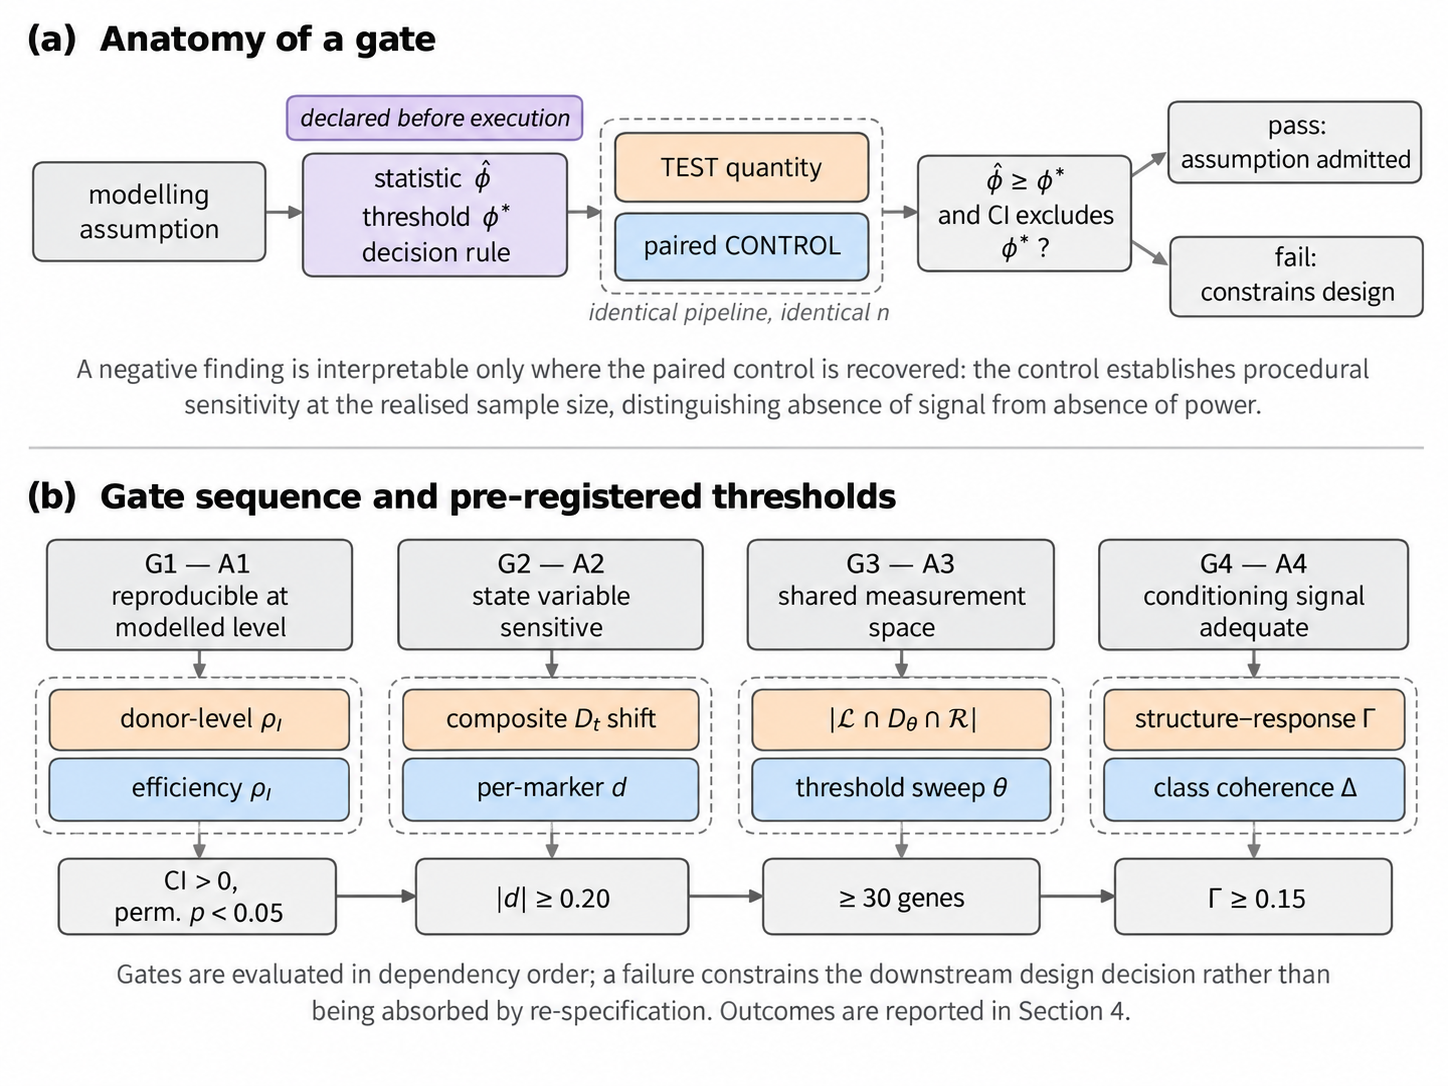
\includegraphics[width=0.70\linewidth]{images/fig1_gate_protocol.png}
  \caption{Control-paired gate protocol. (a) Each gate specifies a statistic, a
threshold, and a decision rule, all declared before execution. A test quantity
and a paired control are measured through an identical pipeline at identical
sample size; recovery of the control establishes procedural sensitivity, which
is what makes a negative finding interpretable. (b) The four gates evaluated
here, with the statistic, paired control, and pre-registered threshold for
each. Gates are evaluated in dependency order and a failure constrains the
downstream design decision rather than being absorbed by re-specification.
Outcomes are reported in Section~\ref{sec:results}.}
  \label{fig:protocol}
\end{figure*}


\begin{table}[!htbp]
\centering
\small
\caption{Symbols used throughout Section 3.}
\begin{tabular}{ll}
\hline
Symbol & Definition \\
\hline
$\mathcal{C}$ & Set of quality-controlled cells \\
$d(c), q(c)$ & Donor and pool identity of cell $c$ \\
$\tau(c), x(c)$ & Timepoint and treatment arm of cell $c$ \\
$\ell(c)$ & Cell-type label of cell $c$ \\
$u=(d,q)$ & Analysis unit (donor--pool combination) \\
$\mathcal{K}$ & Context set $\{D11, D30, D52^-, D52^+\}$ \\
$f_u^{x}$ & Dopaminergic cell fraction in unit $u$, arm $x$ \\
$v_u$ & Perturbation response of unit $u$ \\
$e_u$ & Differentiation efficiency of unit $u$ \\
$\rho_{\mathrm{I}}$ & Intra-class correlation ICC(1,1) \\
$\mathcal{G}_P,\mathcal{G}_D$ & Pluripotency, dopaminergic marker sets \\
$S_t$ & Marker-set score at timepoint $t$ \\
$\mathcal{L}$ & LINCS landmark gene set, $|\mathcal{L}|=978$ \\
$\mathcal{D}_\theta$ & Genes detected above threshold $\theta$ \\
$\mathcal{R},\mathcal{T}$ & Rotenone, tunicamycin reference signatures \\
$\mathbf{z}_a$ & Log-fold-change signature of compound $a$ \\
$\mathbf{m}_a$ & Structural representation of compound $a$ \\
$\sigma(a,b)$ & Structural similarity \\
$r(a,b)$ & Response similarity \\
$\Gamma$ & Structure--response coupling coefficient \\
$\mathcal{M}$ & Mitochondrial compound class, $|\mathcal{M}|=10$ \\
\hline
\end{tabular}
\end{table}
\section{Methodology}

\subsection{\textbf{Study design}}
\label{sec:design}

Four assumptions are made prior to any perturbation model and are tested here
before development rather than assumed. They are:

\begin{itemize}
\item[\textbf{A1}] the response is reproducible at the level at which
prediction is attempted;
\item[\textbf{A2}] the chosen state variable is sensitive to the perturbation;
\item[\textbf{A3}] source and target domains share a measurement space adequate
for transfer;
\item[\textbf{A4}] the conditioning signal carries the information required to
position an unseen perturbation.
\end{itemize}

A precondition $G_0$ precedes these: that the source resources contain the
perturbation and the mechanistic class under study at all. It is evaluated
first, since a failure would render the remaining gates vacuous rather than
informative.

Each assumption is evaluated by a corresponding gate $G_1,\dots,G_4$, specifying
a statistic $\hat{\phi}$, a threshold $\phi^{*}$, and a decision rule fixed and
recorded before the corresponding computation is executed:
\begin{equation}
G_i =
\begin{cases}
\text{pass}, & \hat{\phi}_i \geq \phi_i^{*} \;\wedge\;
               \phi_i^{*} \notin \mathrm{CI}_{95}(\hat{\phi}_i)\\
\text{fail}, & \text{otherwise}
\end{cases}
\label{eq:gate}
\end{equation}

Each negative claim is paired with a control $\hat{\phi}^{+}$: a quantity
established in prior work, measured on identical units through an identical
pipeline at the same sample size. A negative result is admitted only where
$\hat{\phi}^{+}$ is recovered, which establishes procedural sensitivity at the
realised sample size. Controls for $G_1$ and $G_4$ are external quantities
reported independently in the literature; those for $G_2$ and $G_3$ are internal
decompositions of the test statistic, which play the same structural role but do
not constitute independent replication.

Effect sizes with bootstrap intervals are primary and $p$-values secondary,
since several analyses operate at $n$ where negligible effects attain extreme
significance. Gates are evaluated in dependency order and a failure propagates
as a constraint on the downstream design decision rather than being absorbed by
re-specification. The protocol and the four instantiated gates are summarised in
Figure~\ref{fig:protocol}; $G_0$ is a precondition on source availability rather
than a modelling assumption and is reported in Table~\ref{tab:gates} only.

\subsection{\textbf{Datasets}}

\subsubsection{Jerber et al.\ differentiation dataset}
\label{sec:jerber}

Cells were profiled at $\tau \in \{D11, D30, D52\}$
\cite{jerber2021population}, with $0.1\,\mu$M rotenone applied at day 51 for
24\,h to half of each culture, giving $x \in \{-,+\}$ at D52
(Figure~\ref{fig:units}a). The merged object comprises
$|\mathcal{C}| = 1{,}027{,}398$ cells over $32{,}738$ genes.

Categorical encodings differ per source file in both level set and ordering, so
all categoricals were decoded, unioned, and re-encoded; direct code
concatenation would permute $d(c)$ and $x(c)$ silently. Barcodes are unique
within but not across files, so indexing uses the composite key
$(\text{barcode}, \tau)$. Gene ordering was verified identical prior to
concatenation. Expression is library-size normalised with constant row sums,
hence absolute library size is not recoverable.

\begin{figure*}[!htbp]
  \centering
  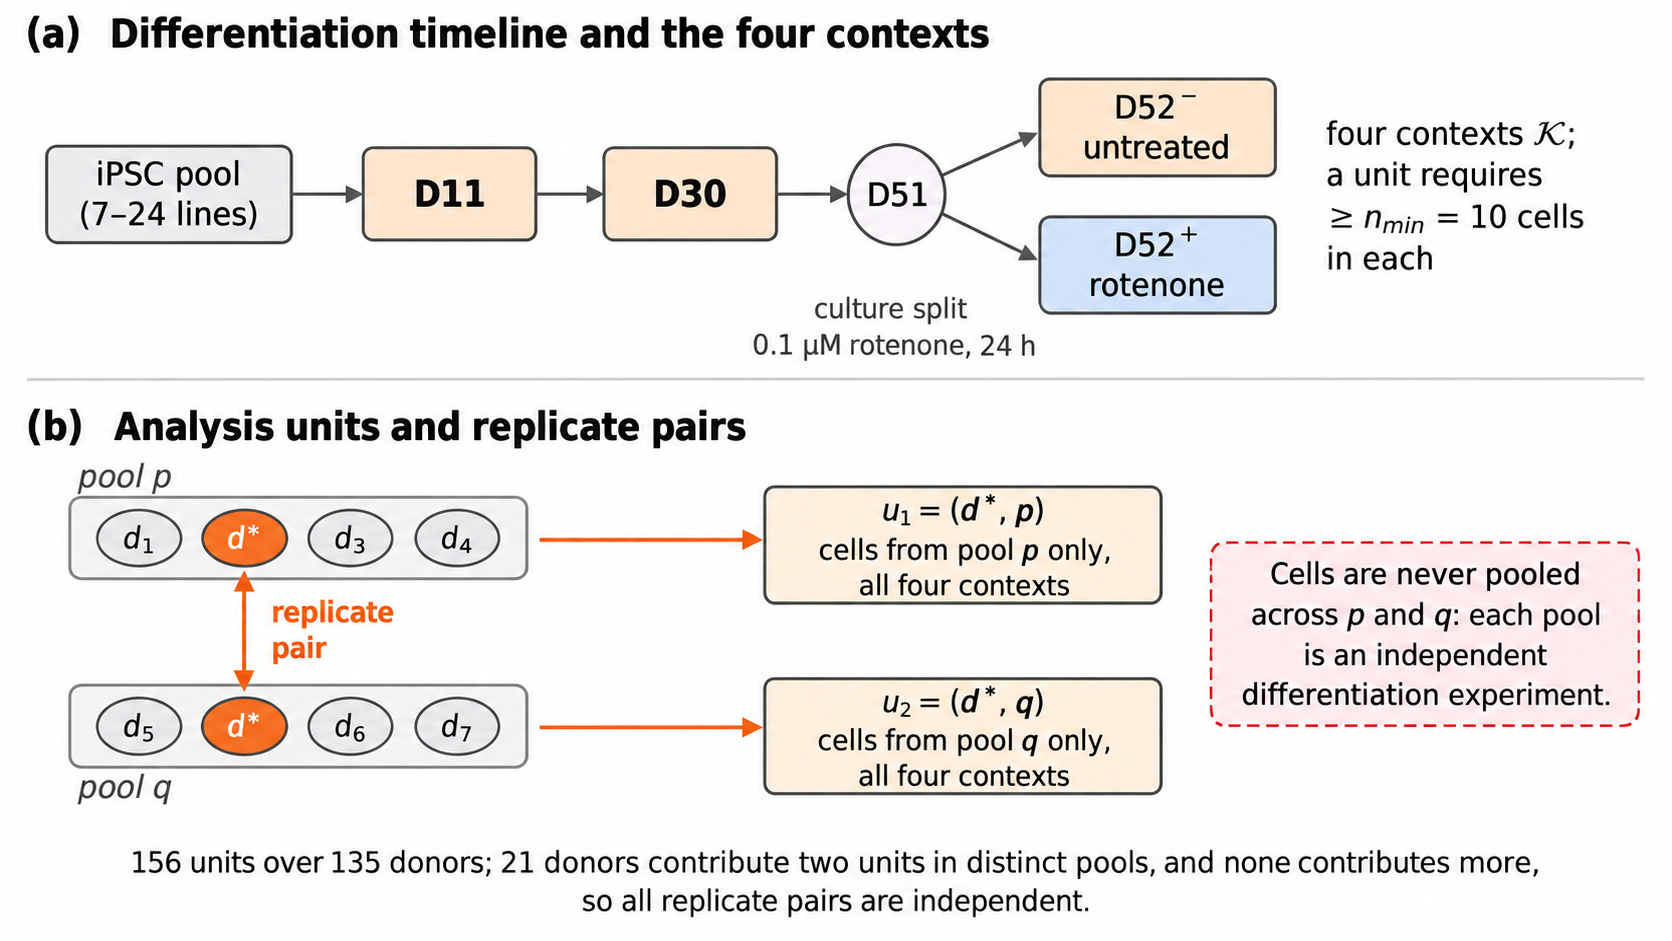
\includegraphics[width=0.65\linewidth]{images/fig2_design_units.png}
  \caption{Experimental design and construction of analysis units. (a) Lines
  are differentiated in pools and profiled at three timepoints; at day 51 each
  culture is split and one arm exposed to rotenone, yielding the four contexts
  a unit must populate. (b) The analysis unit is the (donor, pool) combination
  rather than the donor, since each pool is an independent differentiation
  experiment. A replicate pair arises only where the same line is differentiated
  in two distinct pools, which is rare by design and bounds the sample size
  available to the reproducibility test irrespective of sequencing depth.}
  \label{fig:units}
\end{figure*}

\subsubsection{LINCS L1000}

Level 5 replicate-aggregated signatures over $\mathcal{L}$ were obtained from
GSE92742 \cite{subramanian2017next}. Rotenone is \texttt{BRD-K08316444}
(InChIKey \texttt{JUVIOZPCNVVQFO-HBGVWJBISA-N}); isorotenone and rotenonic acid
resolve to distinct InChIKeys and are excluded. The class $\mathcal{M}$
comprises rotenone, phenformin, metformin, antimycin~A,
thenoyltrifluoroacetone, oligomycin~A, oligomycin~C, CCCP, FCCP, and menadione.

Signatures are filtered on replicate correlation
$\texttt{distil\_cc\_q75} \geq 0.2$, since rotenone carries
$\texttt{is\_touchstone}=0$; unfiltered results are reported alongside.
Structures are admitted only where the parsed SMILES reproduces the annotated
InChIKey.
The precondition $G_0$ is evaluated on this resource: the perturbation must be
represented by at least three replicate-aggregated signatures and the
mechanistic class by at least five distinct structures, thresholds fixed before
the resource was queried.

\subsubsection{Fernandes et al.\ signatures}

Thresholded gene lists $\mathcal{R}$ (rotenone, $1\,\mu$M) and $\mathcal{T}$
(tunicamycin, $5\,\mu$M), both at 24\,h in iPSC-derived dopaminergic neurons,
were taken from \cite{fernandes2020single} (E-MTAB-9154). The wild-type line
KOLF-2 shares HipSci provenance with Section~\ref{sec:jerber}; the datasets are
independent in laboratory, protocol, and dose, but not in cell-line origin.

\subsection{\textbf{State representation}}

For marker set $\mathcal{G}$ and cell $c$ at timepoint $t$,
\begin{equation}
S_t(\mathcal{G}) = \frac{1}{|\mathcal{G}|}\sum_{g\in\mathcal{G}}
\log\!\left(1+\mathrm{expr}_t(g)\right)
\end{equation}
giving $P_t = S_t(\mathcal{G}_P)$ and $D_t = S_t(\mathcal{G}_D)$, with
$\mathcal{G}_P=\{POU5F1,NANOG,SOX2,UTF1,TDGF1\}$ and
$\mathcal{G}_D=\{TH,DDC,SLC6A3,DRD2,LMX1A,FOXA2\}$.

Since $S_t$ is a mean, opposing component shifts cancel: for
$\Delta_g = \mathbb{E}[\mathrm{expr}^+(g)] - \mathbb{E}[\mathrm{expr}^-(g)]$,
$\sum_g \Delta_g \approx 0$ is attainable with $|\Delta_g| \gg 0$ for individual
$g$. This is the mechanism interrogated by $G_2$, and every use of $D_t$ to
characterise perturbation response is accompanied by the per-marker
decomposition $\{\Delta_g\}_{g\in\mathcal{G}_D}$.

\subsection{\textbf{$G_1$ --- reproducibility of donor-level response (A1)}}
\label{sec:gate2}

\paragraph{\textbf{Units}} Cells are never pooled across differentiations, since
each pool constitutes an independent differentiation experiment
(Figure~\ref{fig:units}b). Let
$\mathcal{C}_{u,k}=\{c : (d(c),q(c))=u,\; \kappa(c)=k\}$ for context
$k\in\mathcal{K}$. Unit $u$ is retained iff
\begin{equation}
\min_{k\in\mathcal{K}} |\mathcal{C}_{u,k}| \geq n_{\min}, \qquad n_{\min}=10
\end{equation}
A replicate pair arises only where one line is differentiated in two distinct
pools, a configuration rare by design and therefore bounding the sample size
available to this gate irrespective of sequencing depth.

\paragraph{\textbf{Response and control}} With
$f_u^{x} = |\{c\in\mathcal{C}_{u,D52^x} : \ell(c)=\mathrm{DA}\}| \,/\,
|\mathcal{C}_{u,D52^x}|$,
\begin{equation}
v_u = \log_2\!\frac{f_u^{+}+\epsilon}{f_u^{-}+\epsilon},
\qquad \epsilon = 10^{-3}
\label{eq:v}
\end{equation}
\begin{equation}
e_u = f_u^{-} + s_u^{-}
\label{eq:e}
\end{equation}
where $s_u^{-}$ is the serotonergic fraction in the untreated arm.
Eq.~\eqref{eq:v} is the primary metric, fixed in advance;
$\delta_u = f_u^{+}-f_u^{-}$ is secondary. Eq.~\eqref{eq:e} is the positive
control, established in \cite{jerber2021population} as cell-intrinsic.

\paragraph{\textbf{Reproducibility statistic}} For donors with $\geq 2$ units in
distinct pools, a one-way random-effects model
$y_{ij}=\mu+\alpha_i+\varepsilon_{ij}$ is fitted, where
$\alpha_i\sim\mathcal{N}(0,\sigma_b^2)$ is the donor effect and
$\varepsilon_{ij}\sim\mathcal{N}(0,\sigma_w^2)$ the residual. Then
\begin{equation}
\rho_{\mathrm{I}} = \frac{\sigma_b^2}{\sigma_b^2+\sigma_w^2}
= \frac{\mathrm{MS}_B-\mathrm{MS}_W}{\mathrm{MS}_B+(k-1)\mathrm{MS}_W},
\quad k=2
\label{eq:icc}
\end{equation}
$\rho_{\mathrm{I}}<0$ indicates $\sigma_b^2<\sigma_w^2$: replicates of one donor
disagree more than distinct donors. Eq.~\eqref{eq:icc} is primary as it is
invariant to replicate ordering; Pearson $r$ is reported for comparability with
the published value. The gate threshold is $\mathrm{CI}_{95}(\rho_\mathrm{I})>0$
with permutation $p<0.05$.

\paragraph{\textbf{Inference}} Intervals are obtained by bootstrap over donors,
$B=1000$. The null is
\begin{equation}
\hat{\phi}^{(b)} = \phi\!\left(\pi_b(\mathcal{U})\right), \quad b=1,\dots,1000
\end{equation}
where $\pi_b$ permutes donor identity within pool, preserving pool structure and
all marginals. The analysis is repeated for $n_{\min}\in\{10,20,50\}$ to test
attribution to low-depth estimation noise. Where the gate fails, a one-sided
equivalence bound is applied at $\rho_\mathrm{I} < 0.50$, the conventional
threshold below which reliability is regarded as poor
\cite{koo2016guideline}, using the upper $95$th percentile of the bootstrap
distribution at $B=10{,}000$.

\subsection{\textbf{$G_2$ --- state-variable sensitivity (A2)}}

\paragraph{\textbf{Annotation stability}} Comparison of state within an
annotated population presupposes that the annotation carries the same meaning in
both arms. Reclassification of stressed cells to an ambiguous label would
inflate apparent depletion while purifying the retained population. Labels are
enumerated from data and partitioned into $\{\mathrm{DA}\}$, identified, and
ambiguous. Fractions are compositional, so shifts are analysed under
\begin{equation}
\mathrm{clr}(\mathbf{f})_j = \log f_j - \frac{1}{J}\sum_{i=1}^{J}\log f_i
\end{equation}
which removes the constraint $\sum_j f_j = 1$ under which depletion of one
component mechanically inflates the remainder.

Reclassification and cytotoxicity are separated by their opposing predictions on
retained DA cells. Let $\mu_D^{x}$, $\sigma_D^{x}$ denote the mean and standard
deviation of $D_t$ among cells with $\ell(c)=\mathrm{DA}$ in arm $x$:
\begin{equation}
d = \frac{\mu_D^{+}-\mu_D^{-}}
{\sqrt{\tfrac{1}{2}\left[(\sigma_D^{+})^2+(\sigma_D^{-})^2\right]}}
\label{eq:cohend}
\end{equation}
Reclassification implies $d>0$, since only confidently dopaminergic cells retain
the label; cytotoxicity without relabelling implies $d\approx 0$.
Quality-control fields are compared between arms to establish whether
differential filtering precedes annotation.

\paragraph{\textbf{Sensitivity test}} Conditional on annotation stability, the
gate statistic is Eq.~\eqref{eq:cohend} evaluated on the composite $D_t$,
against a threshold of $|d| \geq 0.20$. The paired control is the same statistic
computed per marker $g \in \mathcal{G}_D$: recovery of substantial per-marker
effects alongside a negligible composite localises the insensitivity in the
aggregation rather than in the perturbation.

\subsection{\textbf{$G_3$ --- transferable gene space (A3)}}
\label{sec:genespace}

Let $\mathcal{D}_\theta = \{g : \Pr[\mathrm{expr}(g)>0] > \theta\}$ evaluated
over DA-labelled D52 cells and required in both arms, for
$\theta\in\{0.01,0.10,0.25\}$. The transferable set is
\begin{equation}
\mathcal{G}^{\ast} = \mathcal{L} \cap \mathcal{D}_\theta \cap \mathcal{R}
\end{equation}
and the rotenone-specific set, excluding generic stress response, is
\begin{equation}
\mathcal{G}^{\mathrm{spec}} = \mathcal{G}^{\ast} \setminus \mathcal{T}
\end{equation}
The gate threshold is $|\mathcal{G}^{\ast}| \geq 30$ at the pre-registered
$\theta = 0.10$. The paired control is the detection sweep over $\theta$, which
establishes that the reported set size reflects a stated detection criterion
rather than an arbitrary one.

\subsection{\textbf{$G_4$ --- structure--response coupling (A4)}}
\label{sec:d1}

A structure-conditioned encoder presupposes that $\sigma(a,b)$ predicts
$r(a,b)$. This is evaluated directly.

\paragraph{\textbf{Representations}} For Morgan fingerprints
$\mathbf{m}\in\{0,1\}^{2048}$ (radius 2),
\begin{equation}
\sigma_{\mathrm{T}}(a,b)=
\frac{\mathbf{m}_a^{\top}\mathbf{m}_b}
{\|\mathbf{m}_a\|^2+\|\mathbf{m}_b\|^2-\mathbf{m}_a^{\top}\mathbf{m}_b}
\end{equation}
For standardised RDKit descriptors $\mathbf{m}\in\mathbb{R}^{200}$,
$\sigma_{\mathrm{C}}(a,b)=\mathbf{m}_a^{\top}\mathbf{m}_b/
(\|\mathbf{m}_a\|\|\mathbf{m}_b\|)$.

\paragraph{\textbf{Coupling}} Pairs are restricted to a common (cell line, dose,
duration) so context is constant. With
$r(a,b)=\rho_S(\mathbf{z}_a,\mathbf{z}_b)$,
\begin{equation}
\Gamma = \rho_S\!\left(
\{\sigma(a,b)\}_{(a,b)\in\mathcal{P}},\;
\{r(a,b)\}_{(a,b)\in\mathcal{P}}\right)
\end{equation}
Pairs sharing a compound are dependent, so intervals are bootstrapped over
compounds, not over $\mathcal{P}$. $\Gamma$ is evaluated in a densely sampled
line for power, in neuronal contexts for relevance, and over both $\mathcal{L}$
and $\mathcal{G}^{\mathrm{spec}}$. The gate threshold is $\Gamma \geq 0.15$.
Because the cheminformatic similarity principle is local rather than global,
mean response similarity is additionally reported for pairs binned by structural
similarity.

\paragraph{\textbf{Class coherence}} Mechanistic annotation does not imply
coherence in response space. With $\mathcal{B}$ a background sample,
$|\mathcal{B}|\geq 100$,
\begin{equation}
\Delta = \frac{1}{|\mathcal{M}|^2}\!\!\sum_{a,b\in\mathcal{M}}\!\! r(a,b)
\;-\;
\frac{1}{|\mathcal{M}||\mathcal{B}|}\!\!\sum_{a\in\mathcal{M}}
\sum_{b\in\mathcal{B}}\!\! r(a,b)
\end{equation}
with significance by permutation of class membership. This is the paired control
for $G_4$: it establishes whether the compound class is detectable in response
space at all, independently of whether structure predicts it.

\paragraph{\textbf{Trivial baseline}} Any learned encoder must exceed
nearest-neighbour retrieval on structure. For held-out $a$ with neighbours
$N_k(a)$ and weights $w_{ab}=\sigma(a,b)$,
\begin{equation}
\hat{\mathbf{z}}_a^{\mathrm{kNN}}=
\frac{\sum_{b\in N_k(a)} w_{ab}\,\mathbf{z}_b}{\sum_{b\in N_k(a)} w_{ab}},
\qquad k\in\{1,3,5,10\}
\end{equation}
against three controls: random neighbours $N_k^{\mathrm{rand}}(a)$; the training
mean $\hat{\mathbf{z}}=|\mathcal{A}|^{-1}\sum_{b\in\mathcal{A}}\mathbf{z}_b$;
and no change $\hat{\mathbf{z}}=\mathbf{0}$. Two regimes are evaluated:
leave-one-compound-out, $\mathcal{A}=\mathcal{A}\setminus\{a\}$; and
leave-one-class-out, $\mathcal{A}=\mathcal{A}\setminus\mathcal{M}$,
corresponding to an unseen mechanism. Scoring is by
$\rho_S(\hat{\mathbf{z}}_a,\mathbf{z}_a)$ and
$\|\hat{\mathbf{z}}_a-\mathbf{z}_a\|_2^2/|\mathcal{G}|$.

\subsection{\textbf{Statistical reporting}}

Intervals are bootstrap percentile, $B=1000$ except where stated, resampled over
the independent unit of each analysis. Paired comparisons use the Wilcoxon
signed-rank test. Permutation nulls shuffle only the label under test,
preserving all marginals. Where $\hat{\phi}$ is negligible but $p$ is extreme,
magnitude governs interpretation and $n$ is reported alongside. Equivalence is
not inferred from $p>\alpha$ alone \cite{lakens2017equivalence}; the paired
control $\hat{\phi}^{+}$ establishes sensitivity, and where a bound is required
it is taken from published interpretation guidance rather than derived from the
observed estimate.

\begin{table*}[!htbp]
  \centering
  \caption{Cohort construction and derived unit counts.}
  \label{tab:cohort}
  \scalebox{0.72}{
  \begin{tabular}{llrrllrrrr}
  \toprule
  Dataset & Accession & Cells & Genes & Timepoints & Treatment arms & Donors & In units & Units$^{\ast}$ & Repl. donors \\
  \midrule
  \cite{jerber2021population} (full) & \texttt{Zenodo 4333872} & 1,027,398 & 32,738 & D11/D30/D52 & NONE, ROT (D52 only) & 215 & 135 & 156 & 21 \\
  \cite{jerber2021population} (20\% subsample) & \texttt{Zenodo 4333872} & 205,416 & 32,738 & D11/D30/D52 & NONE, ROT (D52 only) & 213 & 130 & 150 & 20 \\
  \cite{subramanian2017next} L1000 Phase I & \texttt{GEO GSE92742} & -- & 12,328 & 6 h / 24 h & 20,325 compounds (parsed) & -- & -- & 473,647 & -- \\
  \cite{fernandes2020single} (signatures) & \texttt{E-MTAB-9154} & -- & -- & D52 (DAn1, DAn2) & rotenone, tunicamycin & -- & -- & -- & -- \\
  \bottomrule
  \end{tabular}}
  \begin{minipage}{\linewidth}\footnotesize
  Units are complete (donor, pool) combinations at $n_{\min}=10$ cells in each of the four contexts. \emph{In units} counts donors contributing at least one complete unit; \emph{Repl.\ donors} are those with $\geq 2$ units in distinct pools --- the independent unit for every interval in Table~\ref{tab:repro}. Attrition (cells $\rightarrow$ cells in contexts $\rightarrow$ cells in units $\rightarrow$ units $\rightarrow$ donors $\rightarrow$ replicated donors): 1,027,398 $\rightarrow$ 1,027,398 $\rightarrow$ 901,624 $\rightarrow$ 156 $\rightarrow$ 135 $\rightarrow$ 21. Context assignment discards no cells, since every cell carries a timepoint and a treatment. The chain closes: 21 of the 135 donors contribute two units and none more, so $114 + 2\times21 = 156$. Fernandes et al.\ supplies the rotenone and tunicamycin signatures $\mathcal{R}$ and $\mathcal{T}$ used in Section~4.4; the remaining columns do not apply to it. $^{\ast}$For the differentiation dataset, units are complete (donor, pool) combinations; for L1000 the column reports Level 5 signatures.
  \end{minipage}
\end{table*}

\begin{figure}[!htbp]
  \centering
  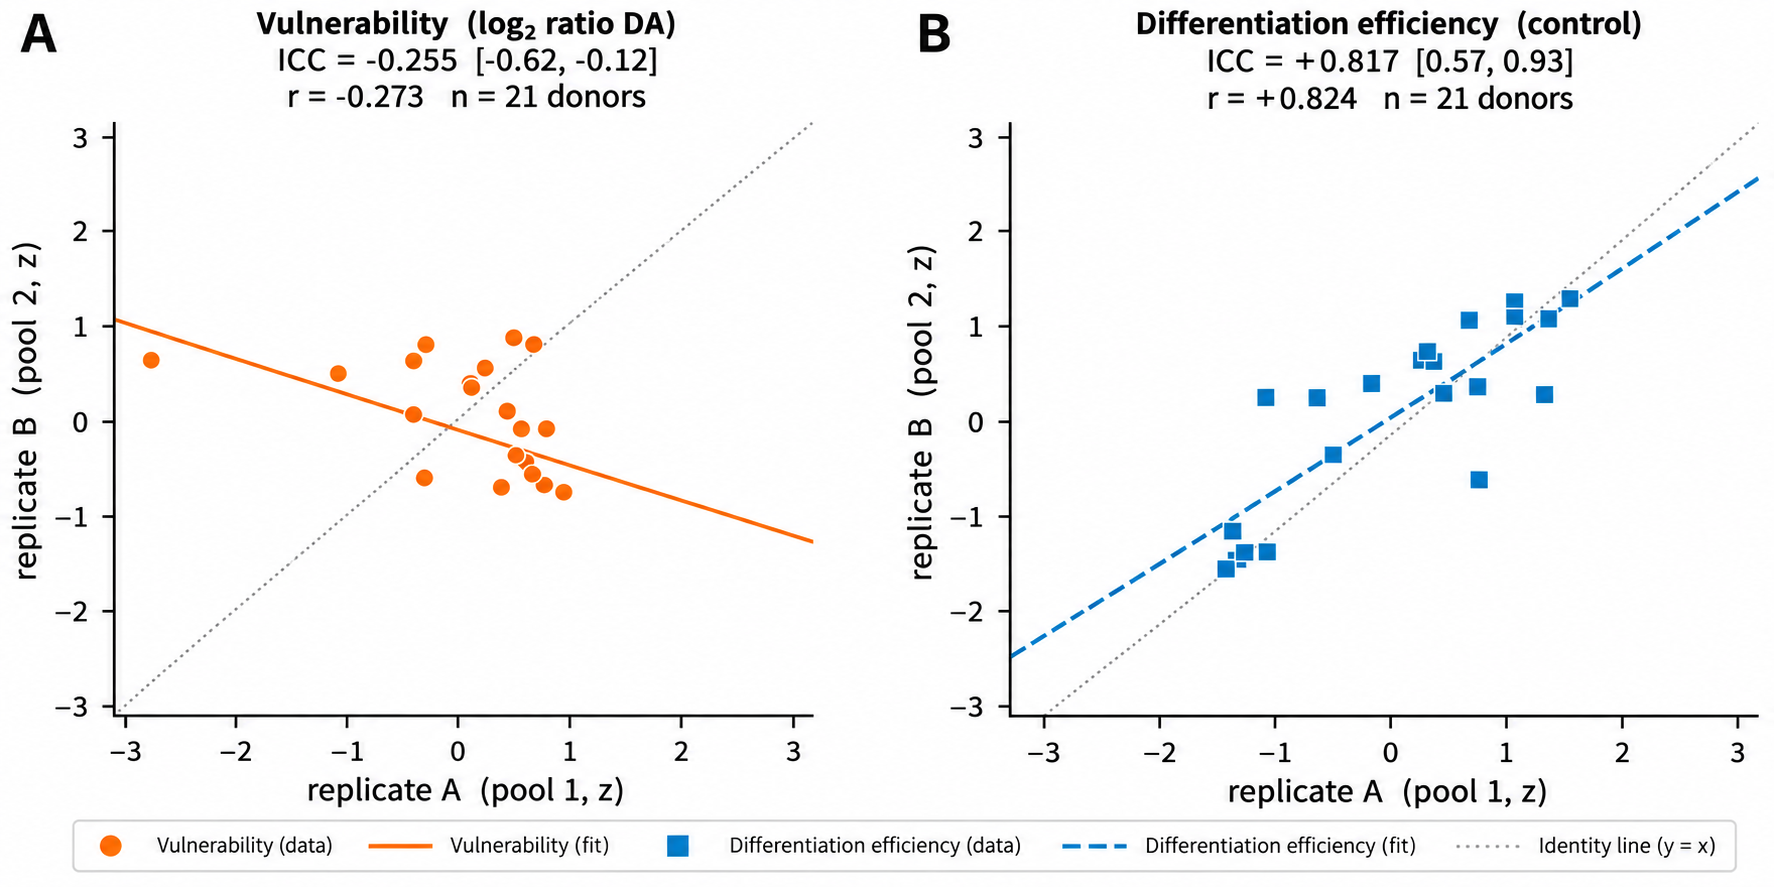
\includegraphics[width=0.99\linewidth]{images/fig2_replicate_scatter.png}
  \caption{Replicate-pair reproducibility for the perturbation response (a) and
  the differentiation-efficiency control (b), on a shared scale with the
  identity line marked. Each point is one donor differentiated in two distinct
  pools; axes are $z$-scored within metric. The control occupies a tight
  diagonal ($\rho_\mathrm{I}=0.817$) while the response forms an uncorrelated
  cloud ($\rho_\mathrm{I}=-0.255$), at identical $n=21$ donors and through an
  identical pipeline. The contrast establishes that the absence of
  reproducibility in (a) reflects the phenotype rather than the sensitivity of
  the procedure.}
  \label{fig:scatter}
\end{figure}



\subsection{\textbf{Reproducibility and pre-specification record}}
\label{sec:repro}

The protocol's central claim, that each threshold was fixed before the
corresponding statistic was computed, is not self-evidencing. The following
record is provided so that the claim can be checked rather than accepted.

\paragraph{\textbf{Pre-specification}} Each gate's statistic, threshold, and
decision rule are declared in the preamble of the script that executes it, and
committed to version control before the commit producing the corresponding
result. The commit history therefore orders declaration before observation, and
that ordering is independently verifiable from the repository timestamps.
% TODO: register the gate specification on OSF or AsPredicted before
% submission and cite the registration identifier here. Repository ordering
% is checkable evidence; an external timestamp is stronger.

\paragraph{\textbf{Data availability}} All three sources are openly accessible
without managed access or data-transfer agreement: the differentiation dataset
via Zenodo (\texttt{doi:10.5281/zenodo.4333872}) and ENA (PRJEB38269), the
chemical perturbation signatures via GEO (GSE92742), and the independent
validation signatures via ArrayExpress (E-MTAB-9154) and the associated
supplementary tables. The analysis is therefore reproducible end to end from
public inputs.

\paragraph{\textbf{Input and output integrity}} Every input file is recorded by
SHA-256 digest together with the commit hash of the processing code. The merged
object of Section~\ref{sec:jerber} is not itself distributed by the source
repository and is produced by a version-controlled merge script whose output
digest is recorded, so that an independently reconstructed object can be
verified against the one analysed here.
% TODO: retain the PureChain provenance layer only if the on-chain anchor of
% the pre-specification digest is reported; otherwise omit this clause.

\paragraph{\textbf{Environment}} The computational environment is specified by a
pinned dependency manifest with resolved versions, verified to install from a
clean interpreter. Analyses fitted with a reference implementation in a second
language, namely the intra-class correlations of Eq.~\eqref{eq:icc}, are
cross-validated against the primary implementation and agreement is reported.

\paragraph{\textbf{Derived artefacts}} The unit table, the replicate-pair table,
and the rotenone-specific gene set $\mathcal{G}^{\mathrm{spec}}$ are released as
tabular files, the last of these being directly reusable independently of the
conclusions drawn here.



\section{\textbf{Results}}
\label{sec:results}

\subsection{\textbf{Cohort and unit construction}}

Table~\ref{tab:cohort} reports cohort construction. The merged object comprises
$1{,}027{,}398$ cells over $32{,}738$ genes across three differentiation
timepoints and two treatment arms. Context assignment discards no cells, as
every cell carries both a timepoint and a treatment label. Requiring
$n_{\min}=10$ cells in each of the four contexts within a single pool retains
$901{,}624$ cells in 156 complete $(d,q)$ units drawn from 135 donors. Of
these, 21 donors contribute two complete units in distinct pools and none
contributes more, so every replicate pair is independent and the 21 donors
constitute the independent unit for all intervals in
Section~\ref{sec:res-repro}.

The replicated-donor count is bounded by experimental design rather than by data
volume. The $20\%$ subsampled release yields 20 replicated donors against 21
here, despite a fivefold increase in cell depth and a rise from 130 to 135 in
donors contributing complete units. Additional sequencing depth from this
resource cannot increase the power of the reproducibility test, and the value
reported here is therefore treated as final.

At D52, $104{,}586$ cells pass quality control, of which $16{,}002$ carry the
dopaminergic label ($10{,}947$ untreated, $5{,}055$ rotenone-treated).

\subsection{\textbf{Donor-level response does not reproduce across differentiations}}
\label{sec:res-repro}

\begin{table*}[!htbp]
  \centering
  \small
  \caption{Donor-level reproducibility of the rotenone response, with the differentiation-efficiency control in the same row group.}
  \label{tab:repro}
  \scalebox{0.78}{
  \begin{tabular}{p{1.2cm} p{4.5cm} p{1.2cm} p{1.2cm} p{3.5cm} p{2cm} p{3.5cm} p{2cm} }
  \toprule
  $n_{\min}$ & Metric & $n$ & $r$ & 95\% CI & $\rho_\mathrm{I}$ & 95\% CI & perm.\ $p$ \\
  \midrule
  10 & $\log_2$ ratio DA (vulnerability) & 21 & -0.273 & [-0.65, -0.11] & -0.255 & [-0.62, -0.12] & 0.147 \\
  10 & $\Delta$ DA fraction & 21 & -0.231 & [-0.54, 0.21] & -0.211 & [-0.40, 0.01] & 0.511 \\
  10 & Diff.\ efficiency \textbf{(control)} & 21 & 0.824 & [0.60, 0.94] & 0.817 & [0.58, 0.93] & $<0.001$ \\
  \midrule
  20 & $\log_2$ ratio DA (vulnerability) & 21 & -0.273 & [-0.65, -0.08] & -0.255 & [-0.62, -0.11] & 0.139 \\
  20 & $\Delta$ DA fraction & 21 & -0.231 & [-0.53, 0.21] & -0.211 & [-0.39, 0.02] & 0.502 \\
  20 & Diff.\ efficiency \textbf{(control)} & 21 & 0.824 & [0.61, 0.95] & 0.817 & [0.59, 0.94] & $<0.001$ \\
  \midrule
  50 & $\log_2$ ratio DA (vulnerability) & 19 & -0.234 & [-0.65, -0.00] & -0.191 & [-0.64, -0.05] & 0.301 \\
  50 & $\Delta$ DA fraction & 19 & -0.081 & [-0.46, 0.35] & -0.109 & [-0.45, 0.07] & 0.866 \\
  50 & Diff.\ efficiency \textbf{(control)} & 19 & 0.824 & [0.59, 0.95] & 0.818 & [0.56, 0.94] & $<0.001$ \\
  \bottomrule
  \end{tabular}}
  \begin{minipage}{\linewidth}\footnotesize
  $n$ is donors with $\geq 2$ complete units in distinct pools --- the independent unit for all intervals. $\rho_\mathrm{I}$ is ICC(1,1). Pre-registered criterion: $\rho_\mathrm{I}$ CI excluding zero on the \emph{positive} side with permutation $p<0.05$. The control reaches $\rho_\mathrm{I}=0.817$ at the same $n$, exceeding the $R=0.75$ ($n=35$) reported by Jerber et al.\ (2021), so the design detects a cell-intrinsic phenotype when one is present. Cross-validated against \texttt{psych::ICC()} (R 4.6.1, psych 2.6.5): agreement to three decimal places on all three metrics. The bootstrap interval describes the sampling distribution of the estimate; the permutation $p$ tests the null of no donor-level structure. A negative $\rho_\mathrm{I}$ arises under that null in approximately half of small samples, so the estimate is interpreted as consistent with absent reproducibility rather than as evidence of negative association. Permutation $p$ is based on 1,000 permutations and is therefore reported as $<0.001$ where no permutation exceeded the observed statistic.
  \end{minipage}
\end{table*}


Table~\ref{tab:repro} and Figure~\ref{fig:scatter} report reproducibility for
the perturbation response and for the control, measured on identical units.

The control reproduces strongly: $\rho_\mathrm{I}=0.817$ (95\% CI
$[0.58,0.93]$), $r=0.824$, permutation $p<10^{-16}$. This exceeds the
$R=0.75$ reported for the same phenotype at $n=35$ in
\cite{jerber2021population}, and establishes that the procedure detects a
cell-intrinsic property of a line at the realised sample size.

The perturbation response does not. Vulnerability yields
$\rho_\mathrm{I}=-0.255$ (95\% CI $[-0.62,-0.12]$), $r=-0.273$, permutation
$p=0.147$; the secondary metric $\Delta$ DA fraction yields
$\rho_\mathrm{I}=-0.211$, $p=0.511$. A negative intra-class correlation
indicates $\sigma_b^2<\sigma_w^2$: two differentiations of one donor agree less
closely than two arbitrary donors. The permutation test does not reject the null
of no donor-level structure, and the estimate is therefore reported as
consistent with absent reproducibility rather than as evidence of a negative
association.

The pre-registered criterion required the interval to exclude zero on the
positive side with permutation $p<0.05$, and is met by neither response metric
at any depth. Raising $n_{\min}$ from 10 to 50 leaves the control unchanged
($0.817 \to 0.818$) while vulnerability remains negative ($-0.255 \to -0.191$),
so the result is not attributable to proportion estimation noise at low cell
counts. Intra-class correlations were cross-validated against an independent
reference implementation with agreement to three decimal places.

Equivalence is established against a one-sided bound rather than inferred from
the permutation result. Taking $\rho_\mathrm{I}<0.50$, the conventional boundary
below which reliability is regarded as poor \cite{koo2016guideline}, the upper
$95\%$ bootstrap limit for vulnerability is $U=-0.145$: donor-level
reproducibility is bounded below any value that would support donor-resolved
prediction. The control does not satisfy the same bound ($U=0.918$) and falls in
the ``good'' band under the same guidance, confirming that the procedure
discriminates rather than admitting every quantity as equivalent.

% TODO --- R2 variance decomposition. Report pool / donor / residual components
% for both metrics (Model A on all 156 units for the pool share; Model B on the
% 42 units from replicated donors for the donor share), and state the
% conclusion positively if pool dominates the response and donor the control.

\subsection{\textbf{Marker composites conceal the transcriptional response}}

\begin{table}[!htbp]
  \centering
  \caption{Per-marker decomposition over $\mathcal{G}_D$, with the composite as the final row.}
  \label{tab:markers}
  \scalebox{0.62}{
  \begin{tabular}{lrrrrllr}
  \toprule
  Marker & NONE & ROT & $\Delta$ & $d$ & 95\% CI & $p$ & \% detected \\
  \midrule
  \textit{TH} & 0.884 & 1.050 & 0.165 & 0.193 & [0.16, 0.23] & $3\times10^{-33}$ & 61.0 / 69.4 \\
  \textit{DDC} & 0.784 & 0.688 & -0.096 & -0.135 & [-0.17, -0.10] & $5\times10^{-14}$ & 61.1 / 56.3 \\
  \textit{SLC6A3} & 0.001 & 0.001 & -0.000 & -0.015 & [-0.05, 0.02] & 0.216 & 0.1 / 0.1 \\
  \textit{DRD2} & 0.118 & 0.128 & 0.009 & 0.029 & [-0.00, 0.06] & 0.581 & 14.6 / 14.6 \\
  \textit{LMX1A} & 0.541 & 0.384 & -0.158 & -0.268 & [-0.30, -0.23] & $6\times10^{-54}$ & 50.1 / 37.4 \\
  \textit{FOXA2} & 0.273 & 0.294 & 0.020 & 0.042 & [0.01, 0.08] & 0.137 & 28.2 / 28.4 \\
  \midrule
  \textbf{$D_t$ (composite)} & 0.434 & 0.424 & -0.010 & -0.039 & [-0.07, -0.01] & 0.060 & 91.4 / 91.1 \\
  \bottomrule
  \end{tabular}}
  \begin{minipage}{\linewidth}\footnotesize
  Within DA-labelled D52 cells; $n=10,947$ NONE and $5,055$ ROT cells (cells are the unit). Values are mean $\log(1+x)$ on CP10K-normalised counts. \emph{\% detected} is NONE / ROT. \textit{TH} rises and \textit{LMX1A} falls; they cancel in the six-marker mean, so the composite $D_t$ is insensitive rather than unchanged. \textit{SLC6A3} is detected in 0.13\% of DA cells and contributes only dilution. As in Table~\ref{tab:repro}, the interval and the $p$-value for the composite ($[-0.07,-0.01]$, $p=0.060$) answer different questions; the magnitude is negligible on either reading and the reported conclusion does not depend on which is taken as primary.
  \end{minipage}
\end{table}

\begin{figure}[!htbp]
  \centering
  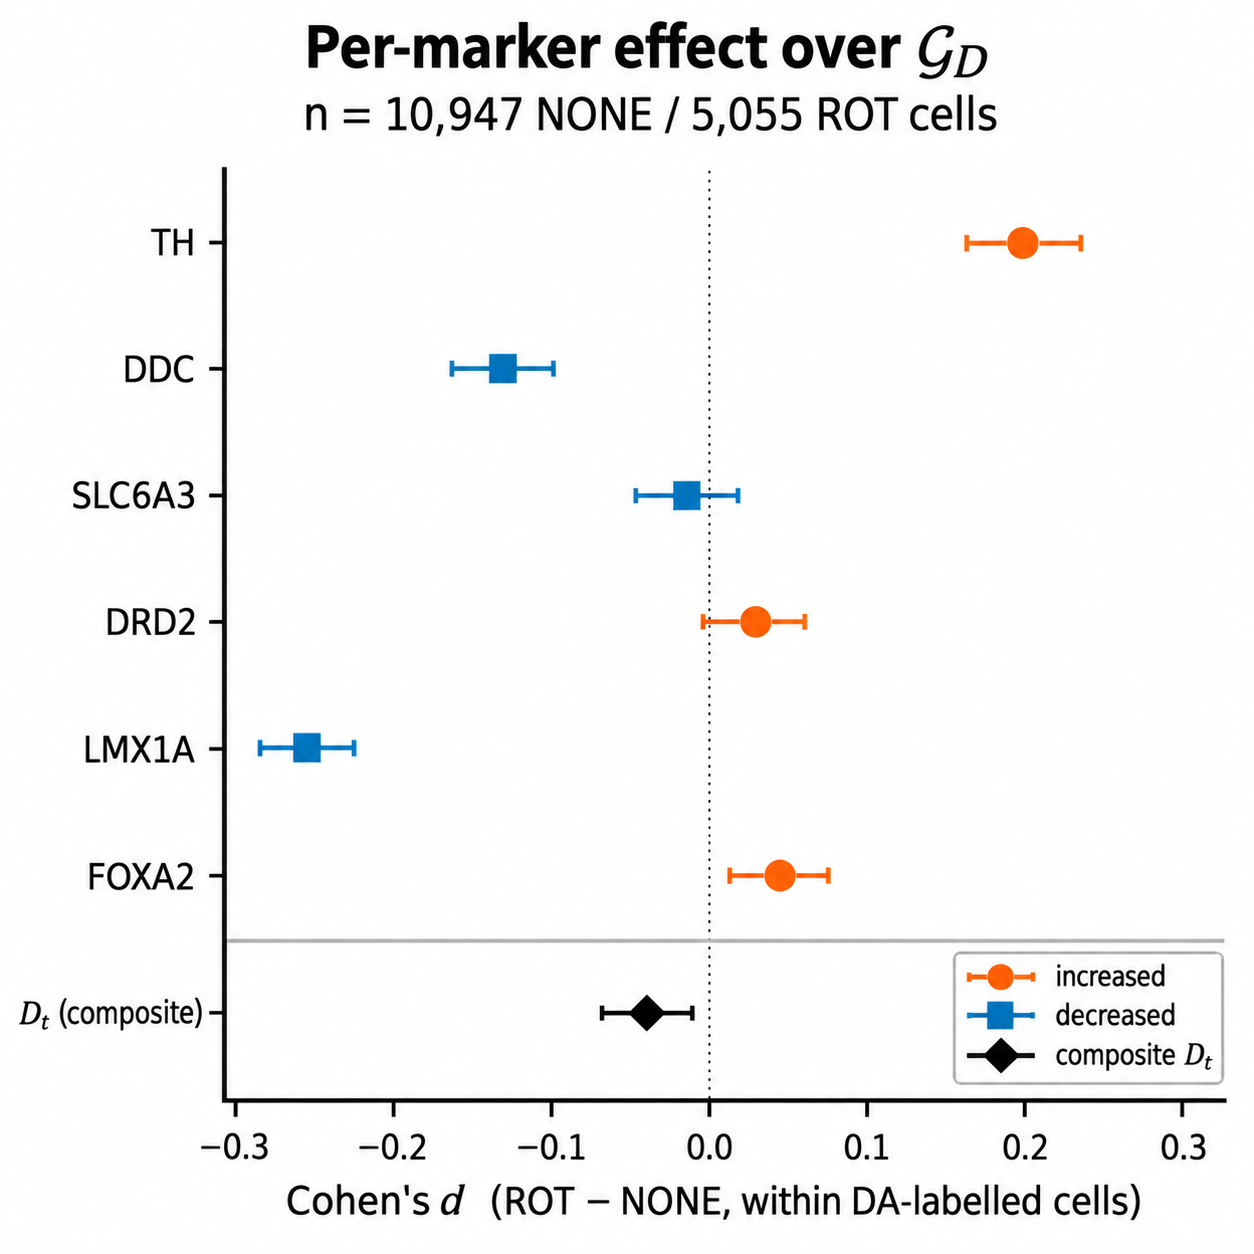
\includegraphics[width=0.65\linewidth]{images/fig3_marker_forest.png}
  \caption{Per-marker effect sizes over $\mathcal{G}_D$ within DA-labelled D52
  cells, with the composite $D_t$ plotted last and separated by a rule.
  \textit{TH} rises and \textit{LMX1A} falls with comparable magnitude and
  opposite sign; averaged over six markers these cancel, leaving the composite
  indistinguishable from no response. Bars are $95\%$ confidence intervals;
  $n=10{,}947$ untreated and $5{,}055$ treated cells.}
  \label{fig:forest}
\end{figure}

\begin{figure}[!htbp]
  \centering
  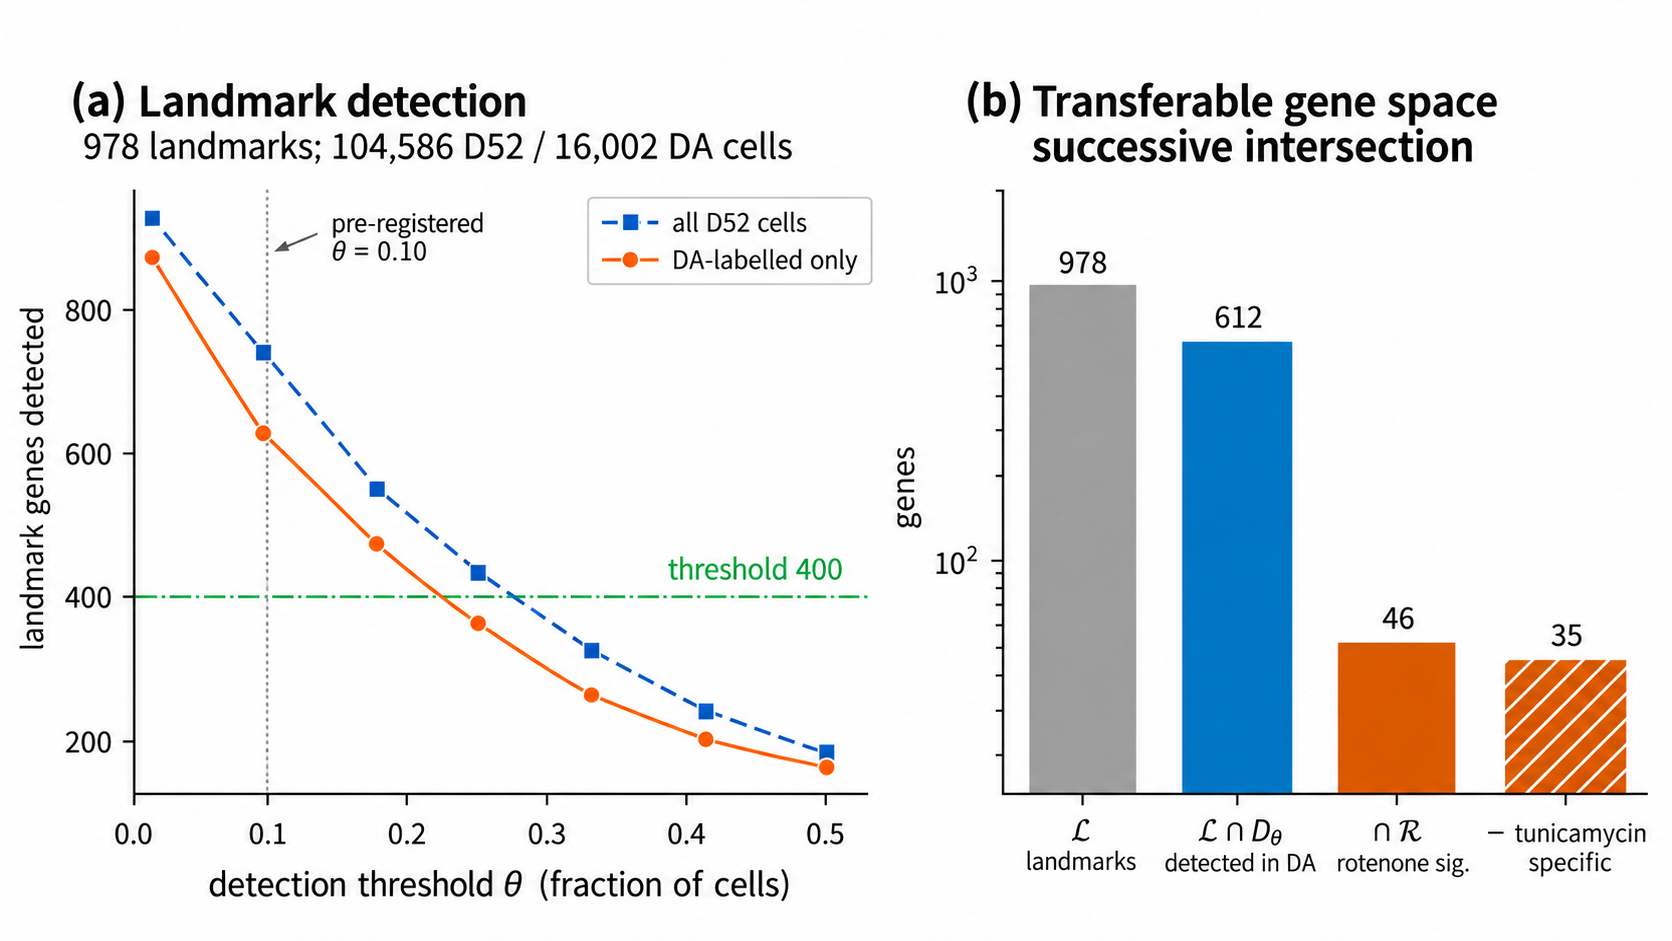
\includegraphics[width=0.95\linewidth]{images/fig4_gene_space.png}
  \caption{(a) Landmark genes detected against detection threshold $\theta$,
  over all D52 cells and over DA-labelled cells only; the pre-registered
  $\theta=0.10$ and the $400$-gene criterion are marked. (b) Successive
  intersection defining the transferable space, from the 978 landmarks to the
  35 genes specific to rotenone after subtraction of the matched tunicamycin
  signature. Note the logarithmic ordinate in (b).}
  \label{fig:genespace}
\end{figure}

Annotation stability was established before interpreting within-population
state, since reclassification of stressed cells would inflate apparent depletion
while purifying the retained population. The ambiguous-label fraction falls
rather than rises under treatment ($-3.43$\,pp), and the composite $D_t$ among
retained dopaminergic cells shifts marginally downward ($d=-0.039$), where
reclassification predicts an upward shift. Mitochondrial fraction also falls,
opposing the elevated-mitochondrial signature of preferentially filtered dying
cells. The annotation is therefore treated as stable across arms, and the
$G_2$ precondition is met.

Under this condition, the composite $D_t$ registers $d=-0.039$ against the
pre-registered threshold of $|d| \geq 0.20$, and $G_2$ therefore fails.
Table~\ref{tab:markers} and Figure~\ref{fig:forest} show that this reflects
cancellation rather than absence. Two markers move substantially and in
opposition: \textit{TH} rises ($d=+0.193$, $p=3\times10^{-33}$) while
\textit{LMX1A} falls ($d=-0.268$, $p=6\times10^{-54}$), with \textit{DDC} also
falling ($d=-0.135$). Averaged over $|\mathcal{G}_D|=6$ markers these contribute
$d=-0.039$ to the composite. The paired control makes the distinction: the same
statistic computed per marker recovers substantial effects in both directions,
so the insensitivity is localised in the aggregation and not in the
perturbation.

Two markers contribute only dilution. \textit{SLC6A3} is detected in $0.13\%$ of
dopaminergic cells and \textit{DRD2} in $14.6\%$, and neither shows a
distinguishable shift. A six-marker mean in which two components are effectively
absent and two move in opposition is structurally insensitive to a
reconfiguration its own constituents record clearly.

This carries a direct methodological consequence. A marker-set composite is a
valid descriptor of differentiation stage, for which its components covary, but
not of perturbation response, for which they need not. Any state variable used
as a prediction target under perturbation requires the per-component
decomposition reported here rather than the composite alone.

\subsection{\textbf{The transferable gene space is small and predominantly downward}}

\begin{table}[!htbp]
  \centering
  \caption{Transferable gene space: successive intersection sizes.}
  \label{tab:genespace}
  \scalebox{0.72}{
  \begin{tabular}{lrrrrrr}
  \toprule
  Signature subset & $|\mathcal{R}|$ & $\cap\,\mathcal{L}$ & $\cap\,\mathcal{D}_\theta$ & Three-way & Arm-stable & Rot.-specific \\
  \midrule
  \texttt{DAn1\_UP} & 200 & 8 & 197 & 7 & 7 & -- \\
  \texttt{DAn2\_UP} & 200 & 7 & 159 & 5 & 5 & -- \\
  \texttt{DAn1\_DE} & 400 & 34 & 389 & 32 & 32 & -- \\
  \texttt{DAn2\_DE} & 400 & 26 & 339 & 22 & 21 & -- \\
  \texttt{UP\_union} & 315 & 13 & 272 & 10 & 10 & -- \\
  \texttt{DE\_union} & 657 & 52 & 587 & 46 & 45 & \textbf{35} \\
  \texttt{DE\_shared} & 143 & 8 & 141 & 8 & 8 & -- \\
  \bottomrule
  \end{tabular}}
  \begin{minipage}{\linewidth}\footnotesize
  $\mathcal{L}$: 978 LINCS landmarks. $\mathcal{D}_\theta$: genes detected in $\geq 10\%$ of 16{,}002 DA-labelled D52 cells ($|\mathcal{L}\cap\mathcal{D}_\theta| = 612$; 561 when required in both arms). Up-regulated signatures alone yield only 7 and 5 genes: the viable space depends on down-regulated genes. The rotenone-specific set is derived by subtracting the tunicamycin signature from the 46-gene three-way intersection, not from the 45 arm-stable genes; 34 of the resulting 35 are arm-stable (\texttt{SOX4} is not).
  \end{minipage}
\end{table}



Table~\ref{tab:genespace} and Figure~\ref{fig:genespace} report the successive
intersection defining genes usable for transfer between the chemical reference
and the dopaminergic system.

Detection threshold dominates the first reduction. Of 978 landmarks, 935 are
detected in $\geq 1\%$ of all D52 cells, but only 612 in $\geq 10\%$ of
dopaminergic cells, and 561 when detection is required in both treatment arms.
The permissive threshold overstates the usable space by approximately $53\%$.

Intersecting with the independent rotenone signature reduces this to 46 genes,
and subtracting the matched tunicamycin signature leaves 35 specific to the
oxidative-stress perturbation rather than to generic stress
(Table~\ref{tab:genelist}); 34 of the 35 are detected stably in both arms. The
retained set contains a coherent mitochondrial and stress-response core
including \textit{CYCS}, \textit{CISD1}, \textit{SLC25A46}, \textit{HSD17B10},
\textit{CYB561}, \textit{HSPB1}, \textit{JUN}, and \textit{SNCA}.

\begin{table}[!htbp]
  \centering
  \caption{The 35 rotenone-specific transferable genes: LINCS landmarks, detected in $\geq 10\%$ of DA-labelled D52 cells, differentially expressed under rotenone, and absent from the tunicamycin signature.}
  \label{tab:genelist}
  \scalebox{0.83}{
  \begin{tabular}{lllll}
  \toprule
  \texttt{ARPP19} & \texttt{ATP6V0B} & \texttt{BLCAP} & \texttt{CAMSAP2} & \texttt{CD320} \\
  \texttt{CHMP6} & \texttt{CISD1} & \texttt{CYB561} & \texttt{CYCS} & \texttt{ELOVL6} \\
  \texttt{FKBP4} & \texttt{GAPDH} & \texttt{HIST2H2BE} & \texttt{HPRT1} & \texttt{HSD17B10} \\
  \texttt{HSPB1} & \texttt{ITGB1BP1} & \texttt{JUN} & \texttt{LYPLA1} & \texttt{MYCBP2} \\
  \texttt{NOSIP} & \texttt{NPDC1} & \texttt{PAFAH1B1} & \texttt{PCMT1} & \texttt{PGRMC1} \\
  \texttt{PIN1} & \texttt{PKIG} & \texttt{PSMB10} & \texttt{RHEB} & \texttt{RPS5} \\
  \texttt{SLC25A46} & \texttt{SLC2A6} & \texttt{SNCA} & \texttt{SOX4} & \texttt{TCTA} \\
  \bottomrule
  \end{tabular}}
  \begin{minipage}{\linewidth}\footnotesize
  All 35 are landmarks and 34 are arm-stable (\texttt{SOX4} is not).
  \end{minipage}
\end{table}

Direction is decisive. Restricting to up-regulated genes yields only 7 and 5
genes for the two neuronal subtypes, against 32 and 22 for the full
differentially expressed lists. A transferable representation of the rotenone
response in this system depends on down-regulated genes.
\begin{figure*}[!htbp]
  \centering
  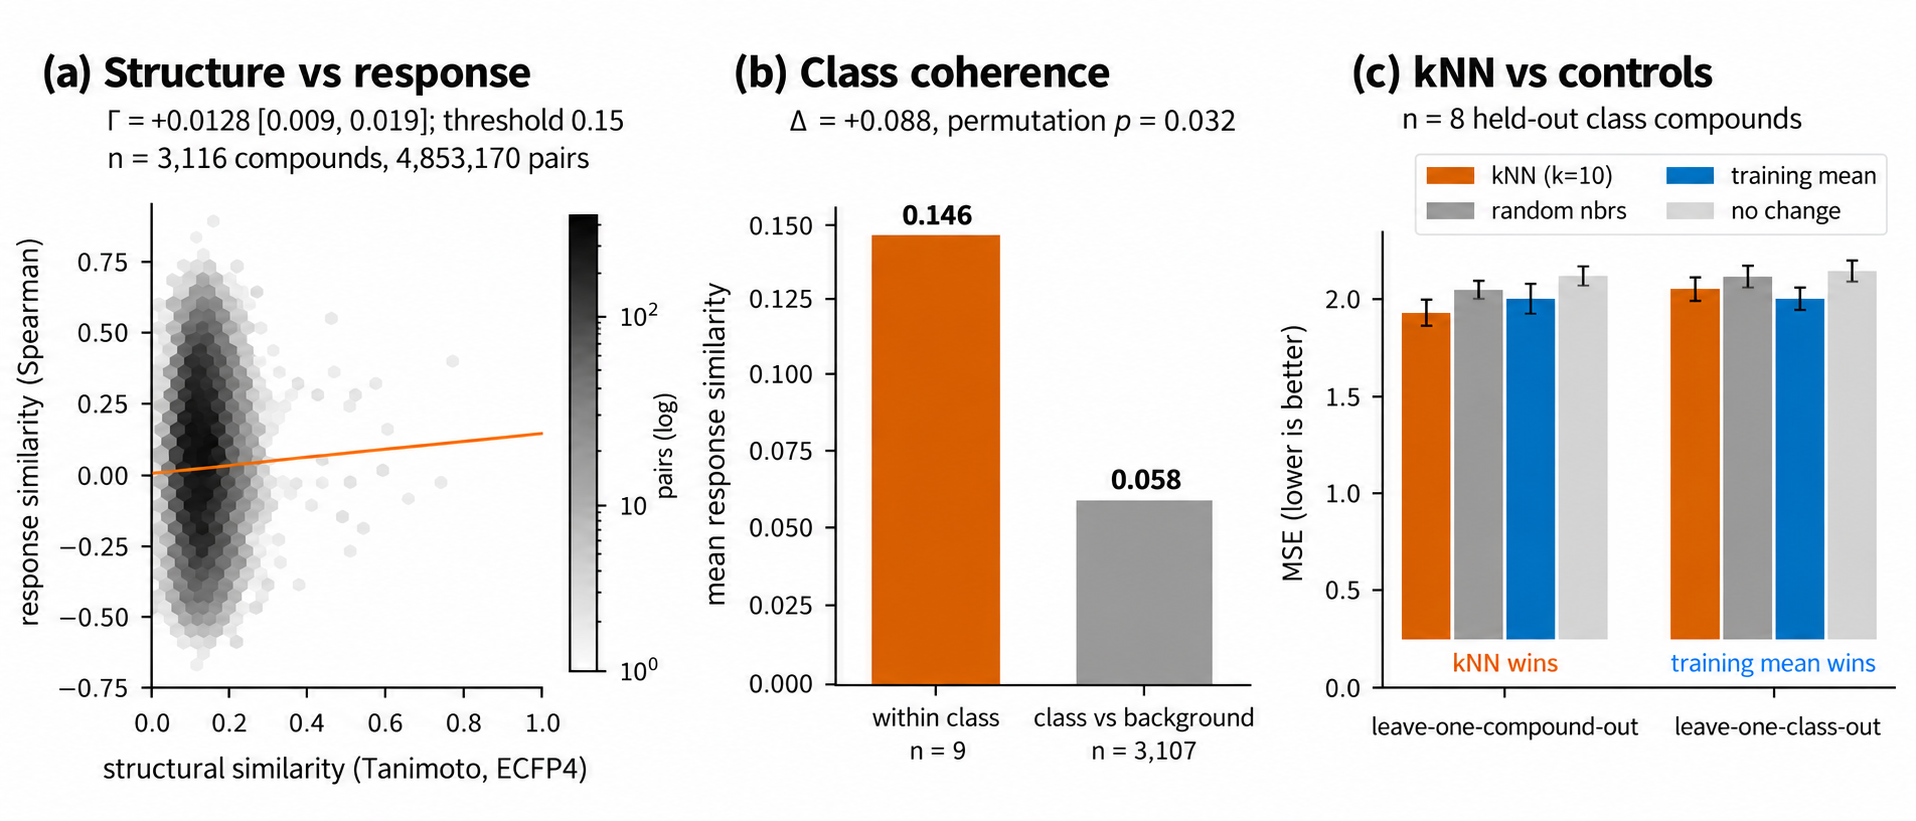
\includegraphics[width=0.76\linewidth]{images/fig5_structure_response.png}
  \caption{(a) Structural against response similarity over all within-context
  compound pairs; the fitted trend and coupling coefficient $\Gamma$ are
  annotated against the pre-registered threshold of $0.15$. (b) Mean signature
  similarity within the mitochondrial class against class-versus-background,
  with permutation significance. (c) Nearest-neighbour prediction error against
  three controls under two holdout regimes. Retrieval on structure outperforms
  all controls when a single compound is withheld and close analogues remain in
  the pool, but is beaten by the training mean when the entire mechanistic class
  is withheld. Lower is better in (c).}
  \label{fig:coupling}
\end{figure*}



The dopaminergic identity axis is not transferable at all. \textit{TH} and
\textit{DDC} are absent from the LINCS gene space entirely, and
\textit{ALDH1A1}, \textit{COMT}, and \textit{NR4A2} are present only as inferred
rather than directly measured genes. A model pretrained on this resource cannot
emit a dopamine-synthesis readout, independently of its architecture.

\begin{table*}[!htbp]
  \centering
  \small
  \caption{Structure--response coupling by representation, context and gene space, against the pre-registered threshold.}
  \label{tab:coupling}
  \scalebox{0.70}{
  \begin{tabular}{p{4.3cm} p{2.5cm} p{2.5cm} p{1.5cm} p{1.5cm} p{1.5cm} p{2.5cm} p{1.5cm}}
  \toprule
  Context & Gene space & Repr. & Cpds. & Pairs & $\Gamma$ & 95\% CI & Threshold \\
  \midrule
  MCF7 10.0$\,\mu$M 24h & landmark978 & \texttt{morgan} & 3,116 & 4,853,170 & +0.0128 & [0.009, 0.019] & 0.15 \\
   & landmark978 & \texttt{rdkit\_desc} & 3,116 & 4,853,170 & +0.0112 & [0.008, 0.016] & 0.15 \\
   & specific35 & \texttt{morgan} & 3,116 & 4,853,170 & +0.0104 & [0.005, 0.017] & 0.15 \\
   & specific35 & \texttt{rdkit\_desc} & 3,116 & 4,853,170 & +0.0085 & [0.006, 0.014] & 0.15 \\
  \midrule
  NPC 10.0$\,\mu$M 24h$^{\dagger}$ & landmark978 & \texttt{morgan} & 1,394 & 970,921 & +0.0119 & [0.008, 0.021] & 0.15 \\
   & landmark978 & \texttt{rdkit\_desc} & 1,394 & 970,921 & -0.0041 & [-0.007, 0.005] & 0.15 \\
   & specific35 & \texttt{morgan} & 1,394 & 970,921 & +0.0180 & [0.010, 0.030] & 0.15 \\
   & specific35 & \texttt{rdkit\_desc} & 1,394 & 970,921 & -0.0076 & [-0.012, 0.003] & 0.15 \\
  \midrule
  NEU 10.0$\,\mu$M 6h$^{\dagger}$ & landmark978 & \texttt{morgan} & 280 & 39,060 & +0.0277 & [0.022, 0.059] & 0.15 \\
   & landmark978 & \texttt{rdkit\_desc} & 280 & 39,060 & +0.0350 & [0.021, 0.079] & 0.15 \\
   & specific35 & \texttt{morgan} & 280 & 39,060 & +0.0302 & [0.016, 0.070] & 0.15 \\
   & specific35 & \texttt{rdkit\_desc} & 280 & 39,060 & +0.0207 & [0.002, 0.062] & 0.15 \\
  \bottomrule
  \end{tabular}}
  \begin{minipage}{\linewidth}\footnotesize 
  $\Gamma$ is the Spearman correlation between structural similarity and signature similarity over all within-context compound pairs; intervals bootstrap over \emph{compounds}, since pairs share compounds and are not independent. No representation in any context reaches the pre-registered 0.15. Extreme $p$-values (to $3\times10^{-174}$) reflect $n=4.85$M pairs, not effect size: $\Gamma=0.0128$ corresponds to $\approx 0.02\%$ of variance explained. $^{\dagger}$neuronal context, underpowered.
  \end{minipage}
\end{table*}

\begin{table*}[!htbp]
  \centering
  \small
  \caption{Pre-registered gate outcomes. Each threshold was fixed before the corresponding computation; negative findings are reported against a paired control measured through the same procedure at the same sample size.}
  \label{tab:gates}
  \scalebox{0.75}{
  \begin{tabular}{p{3.4cm} p{4.8cm} p{3.2cm} p{3.5cm} p{2.6cm} l}
  \toprule
  Gate & Question & Threshold & Observed & Paired control & Verdict \\
  \midrule
  $G_0$ & Rotenone represented in source? & $\geq 3$ signatures & 77 (56 lines) & --- & pass \\
   & Mechanistic class available? & $\geq 5$ compounds & 10 & --- & pass \\
  \midrule
  $G_1$ (A1) & Response reproduces across differentiations? & $\rho_\mathrm{I}$ CI $>0$, perm.\ $p<0.05$ & $-0.255$ $[-0.62,-0.12]$, $p=0.147$ & $0.817$ $[0.58,0.93]$ & \textbf{fail} \\
   & Reproducibility bounded below usable? & $U < 0.50$ (Koo \& Li) & $U=-0.145$ & $U=0.918$ (not met) & \textbf{equiv.} \\
  \midrule
  \multicolumn{6}{@{}l}{\emph{$G_2$ precondition}} \\
   & Annotation stable under treatment? & ambiguous rise $<2$\,pp & $-3.43$\,pp & --- & pass \\
   &  & within-DA $|d|<0.2$ & $-0.039$ & --- & pass \\
  $G_2$ (A2) & Composite sensitive to perturbation? & $|d| \geq 0.20$ & $-0.039$ & per-marker $+0.193$ / $-0.268$ & \textbf{fail} \\
  \midrule
  $G_3$ (A3) & Landmarks detected in DA cells? & $\geq 400$ at $\theta=0.10$ & 612 & sweep over $\theta$ & pass \\
   & Rotenone-responsive intersection? & $\geq 30$ genes & 46 (35 specific) & --- & pass \\
  \midrule
  $G_4$ (A4) & Structure predicts response? & $\Gamma \geq 0.15$ & $+0.0128$ $[0.009,0.019]$ & $\Delta=+0.088$, $p=0.032$ & \textbf{fail} \\
   & Trivial baseline strength & (recorded, no threshold) & kNN wins LOCO; training mean wins LOCLASS & --- & --- \\
  \bottomrule
  \end{tabular}}
  \begin{minipage}{\linewidth}\footnotesize
  Every threshold was fixed before the corresponding computation and none was adjusted afterwards. $G_1$ intervals use donors ($n=21$) as the independent unit. The equivalence row applies a one-sided bound at $\rho_\mathrm{I}<0.50$, the poor/moderate boundary of \cite{koo2016guideline}; the control fails the same bound, which shows the test discriminates. The $G_2$ precondition and the $G_2$ gate evaluate the same statistic against opposite criteria: a small within-DA $|d|$ establishes that stressed cells are not being relabelled, and simultaneously that the composite does not register the perturbation. $G_0$ establishes that the data required to validate a compound encoder exist; $G_4$ establishes that the premise such a validation rests on does not hold --- the two are not in conflict.
  \end{minipage}
\end{table*}

\subsection{\textbf{Structural similarity does not predict response across mechanisms}}

Table~\ref{tab:coupling} reports the structure--response coupling $\Gamma$
across representations, contexts, and gene spaces. No configuration approaches
the pre-registered threshold of $0.15$. In the densely sampled context the
strongest estimate is $\Gamma=+0.0128$ (95\% CI $[0.009,0.019]$) over
$3{,}116$ compounds and $4{,}853{,}170$ pairs, corresponding to approximately
$0.02\%$ of variance in response similarity. Extreme $p$-values, to
$3\times10^{-174}$, reflect pair count rather than effect magnitude. Neuronal
contexts return estimates of comparable magnitude, reaching $+0.035$ at $n=280$
compounds, and are reported as underpowered. Descriptor and fingerprint
representations perform equivalently, with the descriptor estimate crossing zero
in one context.

Two further results locate the failure precisely.

First, the compound class is coherent in response space. Within-class mean
signature similarity is $0.146$ against $0.058$ for class-versus-background,
$\Delta=+0.088$, permutation $p=0.032$ (Figure~\ref{fig:coupling}b). Compounds
sharing a mechanism converge transcriptionally even where they share no
scaffold.


\begin{figure}[!htbp]
  \centering
  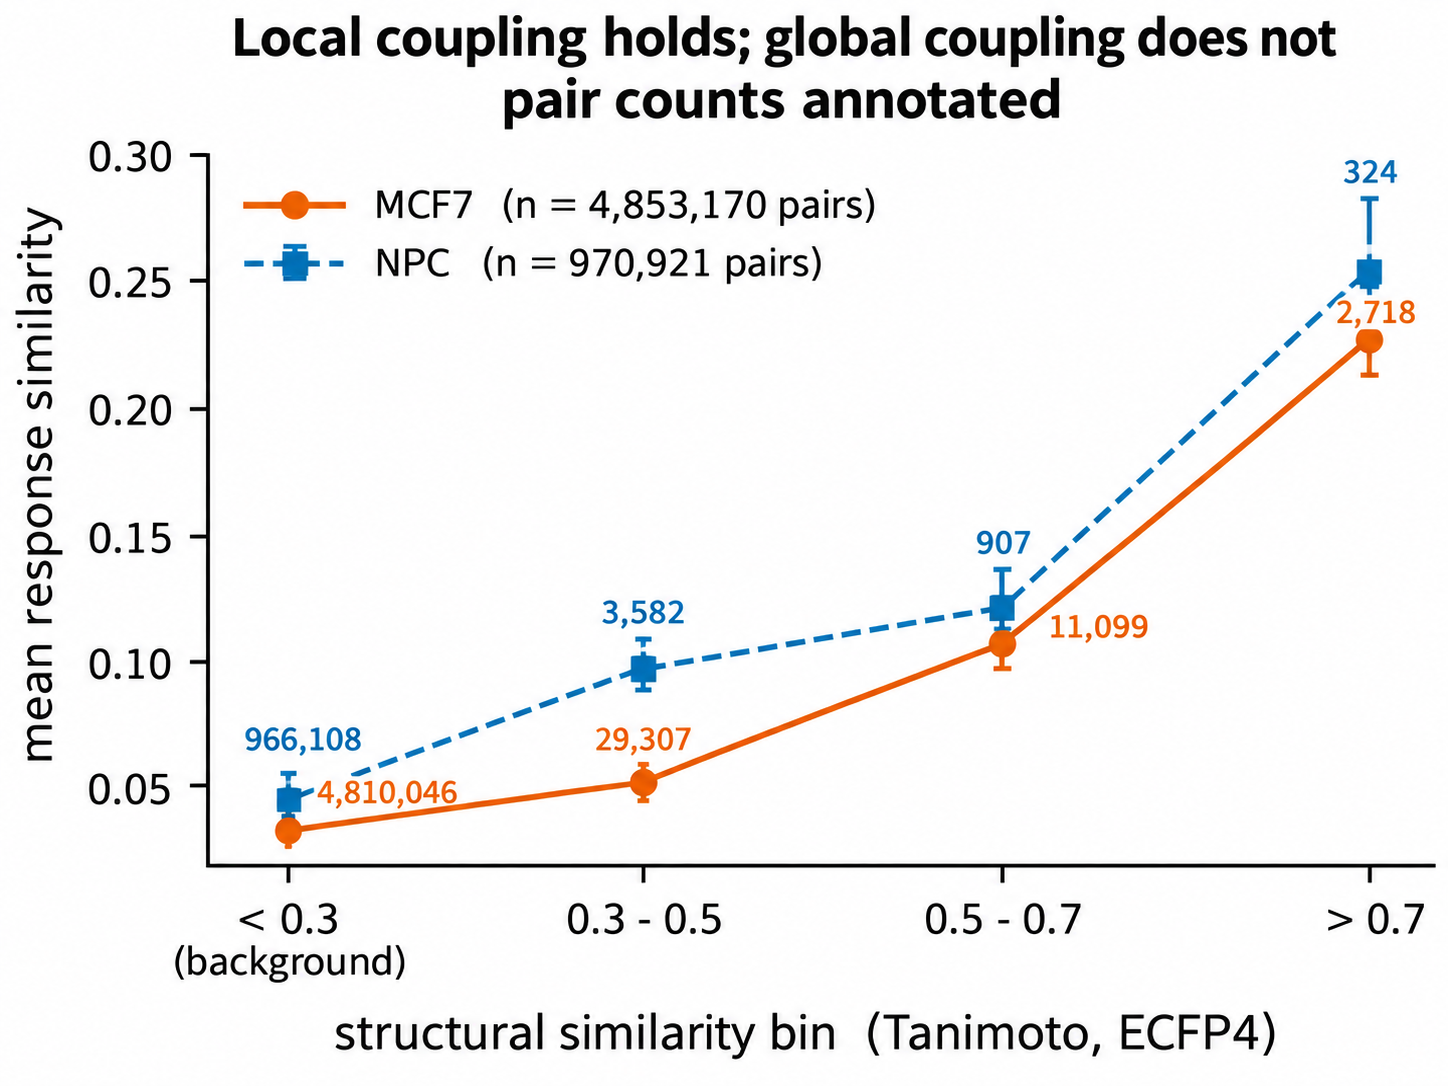
\includegraphics[width=0.78\linewidth]{images/fig6_stratified_similarity.png}
  \caption{Mean response similarity by structural similarity band, with pair
  counts annotated. The relation is monotone and strong among near-analogues
  ($T>0.7$) and vanishes into the background-dominated majority of pairs, which
  is why the global coupling coefficient of Table~\ref{tab:coupling} is
  negligible despite a real local association.}
  \label{fig:stratified}
\end{figure}

Second, structural similarity does predict response, but only locally.
Figure~\ref{fig:stratified} stratifies pairs by structural similarity: mean
response similarity rises monotonically from $0.032$ at background ($T<0.3$) to
$0.228$ at $T>0.7$ in the densely sampled context, and from $0.045$ to $0.253$
in the neuronal context, approximately sevenfold and sixfold elevations. The
relation holds among near-analogues and vanishes across the population, which is
why the global coefficient is negligible.

The consequence is visible in the trivial baseline
(Figure~\ref{fig:coupling}c). Under leave-one-compound-out, nearest-neighbour
retrieval on structure outperforms all controls, because close analogues remain
in the pool. Under leave-one-class-out, where the entire mitochondrial class is
withheld and no analogue remains, the training mean is the better predictor.
Structure-conditioned retrieval therefore generalises to an unseen compound but
not to an unseen mechanism.

Taken together: mechanism predicts response, and structure predicts mechanism
only among near-analogues. A structure-conditioned encoder trained on this
resource has no basis on which to position a compound whose mechanistic class is
unrepresented in training.

\subsection{\textbf{Feasibility summary}}

Table~\ref{tab:gates} collects every gate outcome against its pre-registered
threshold. The following constraints follow, each established against a
threshold fixed in advance and, where the finding is negative, against a paired
control measured through the same procedure at the same sample size.

Donor-resolved prediction of perturbation response is not supported: the
response does not reproduce across differentiations of the same line, while a
developmental phenotype measured identically does, and reproducibility is
bounded below any usable value. Marker-set composites are not valid prediction
targets under perturbation, as they cancel opposing component shifts. The
transferable gene space is 35 genes rather than the several hundred implied by
permissive detection thresholds, and excludes the dopaminergic identity axis
entirely. Structure-conditioned transfer does not generalise across mechanistic
classes, although mechanistic class is itself transcriptionally coherent and
structural similarity is predictive among near-analogues.

\section{\textbf{Discussion}}
 
\subsection{\textbf{Where the failures occur}}
 
Three of the four assumptions fail, and all three fail at the level of the data
rather than the model: no architecture, training budget, or representation
recovers a phenotype that does not reproduce, a state variable that cancels its
own components, or a conditioning signal that does not span the space it is
asked to generalise over. This is the pattern the protocol was designed to
expose, and it is not visible to a benchmark comparison, which can only report
that a model fails to beat a baseline without identifying why.
 
The finding therefore complements rather than competes with the recent
benchmarking literature. Deep models are reported to fall short of trivial
predictors across genetic \cite{ahlmann2025deep} and chemical
\cite{wu2026perturbench, radig2026scarchon} perturbation tasks. One contributing
explanation is supplied here: where the premises of the task do not hold, a
model has nothing to learn beyond the marginal, and predicting the training
mean is the rational limit of its behaviour. Read this way, mode collapse
\cite{mejia2025diversity} is in part a symptom of task specification rather
than solely of model or metric design.
 
The $G_4$ result carries a sharper implication. Structural similarity predicts
transcriptional response strongly among near-analogues and negligibly across
the population, and the trivial baseline wins under leave-one-compound-out
while losing under leave-one-class-out (Figure~\ref{fig:coupling}c). A
structure-conditioned encoder evaluated only on held-out compounds may
therefore be performing retrieval over close analogues retained in training
rather than generalisation, and would report success under an evaluation that
never withholds a mechanistic class. Holding out the class, not the compound,
is what distinguishes the two.

\subsection{\textbf{Limitations}}

The findings are bounded in three ways. The case comprises one resource and one
compound at a single dose and duration, so the specific failures at $G_1$ and
$G_2$ are properties of a sub-lethal oxidative challenge in this system; the
protocol, not the findings, is what transfers. The reproducibility test rests on
21 replicated donors, a ceiling imposed by an experimental design in which few
lines are differentiated twice rather than by the data available, so the
conclusion is carried by the equivalence bound rather than by the point
estimate. And the controls for $G_2$ and $G_3$ are internal decompositions
rather than independently established quantities: they show that the measurement
is not uniformly null, but the corresponding negatives are weaker than those for
$G_1$ and $G_4$.

Two measurement constraints are noted rather than resolved. The analysed object
is library-size normalised, so all reported shifts are relative and recovering
absolute change would require reprocessing from raw counts. Neuronal signatures
for the compound class exist only at $10\,\mu$M, two orders above the modelled
exposure, so the $G_4$ verdict is carried by the densely sampled context.

\subsection{\textbf{Implications for digital twin construction}}

The gates are diagnostic rather than merely prohibitive: each verdict prescribes
a property the eventual model must have. Because the response is not a stable
property of the cell line, $G_1$ fixes the aggregation level, requiring that a
twin for this system predict the population-average response rather than
condition on donor, since donor conditioning would fit variance belonging to the
differentiation batch. $G_2$ fixes the state variable: a composite marker score
is an adequate coordinate for differentiation stage, where its components
covary, but not for prediction under perturbation, where they need not, so
perturbation-responsive dimensions must be carried at component resolution.
$G_3$ fixes the output space, which is 35 genes and excludes the
dopamine-synthesis axis, so a twin consuming a bulk chemical reference must emit
predictions in a stress-response space and cannot be evaluated against a
dopaminergic-identity readout however desirable that target is. And $G_4$ fixes
both the conditioning signal and the evaluation: structure supports
interpolation among near-analogues but not extrapolation to unseen mechanisms,
while mechanism itself is coherent in response space, so conditioning should
incorporate mechanistic information and leave-one-class-out should be reported
alongside leave-one-compound-out as a matter of course.

Composed, these prescribe a digital twin that is population-level rather than
donor-resolved, targets components rather than composites, predicts into a
defined stress-response gene space, conditions on mechanism as well as
structure, and is evaluated with a mechanism-level holdout. Where a gate
identifies a limit of the data rather than of the design, it equally specifies
what a future resource must supply: donor-resolved prediction requires lines
differentiated repeatedly, sized so that the replicate count is not the binding
constraint, and a dopaminergic-identity readout requires a chemical reference
that measures those genes rather than a different architecture. None of these
constraints could have been derived from a benchmark comparison, and each would
otherwise have been discovered only after the corresponding model had been
built. This is the sense in which the protocol guides construction rather than
merely licensing or refusing it.

\section{Conclusion}

This work tested four assumptions that precede any perturbation model, under a
protocol in which each statistic and threshold was fixed before computation and
each negative finding anchored to a control measured through an identical
pipeline. Three of the four fail on a widely used iPSC-derived dopaminergic
resource. Donor-level response does not reproduce across independent
differentiations ($\rho_\mathrm{I}=-0.255$) while a developmental phenotype
measured identically does ($\rho_\mathrm{I}=0.817$), bounding prediction to the
population average; a canonical marker composite is insensitive to a
perturbation its own components register clearly, and is therefore not a valid
target; and structural similarity predicts transcriptional response among
near-analogues but not across mechanistic classes ($\Gamma=0.0128$), although
mechanistic class is itself coherent in response space. The single assumption
that holds yields a transferable space of 35 genes, an order of magnitude
smaller than permissive detection thresholds imply and excluding the
dopaminergic identity axis entirely. Each failure is localised to a specific
stage rather than reported as an aggregate inability to fit a model, and the
paired controls establish that these are properties of the data rather than of
the procedure.

Two directions follow. Within this system, the constraints identified here are
not uniformly permanent: the bound on donor-level analysis is imposed by an
experimental design in which few lines are differentiated more than once, and
would be lifted by a resource with replicated differentiations, whereas the
absence of a dopamine-synthesis readout in bulk chemical references and the
scarcity of compounds assayed in both a chemical library and a dopaminergic
context are constraints on the reference data rather than on the method. Beyond
this system, the protocol is independent of the case to which it was applied,
and the control-pairing requirement transfers directly to any setting in which a
model is to be built on an untested assumption. Its value is greatest where the
cost of discovering an unsupported premise after development is highest, which
in perturbation modelling is the common case.
%%────────────────────────────────────────────────────────────────────
\section*{Acknowledgment}

%%────────────────────────────────────────────────────────────────────
This work was partly supported by Innovative Human Resource Development for Local Intellectualization program through the IITP grant funded by the Korea government (MSIT) (IITP-2026-RS-2020-II201612, 33\%) and by Priority Research Centers Program through the NRF funded by the MEST (2018R1A6A1A03024003, 33\%) and by the MSIT, Korea, under the ITRC support program (IITP-2026-RS-2024-00438430, 34\%),  and the Regional Innovation System \& Education (RISE) (Regional Growth Innovation LAB) program through the Gyeongbuk RISE Center, funded by the Ministry of Education (MOE) and the Gyeongsangbuk-do, Republic of Korea (2025-rise-15-105).


\small
\bibliographystyle{elsarticle-num}
\vspace{-0.3cm}
\bibliography{newref}
\vspace{-0.3cm}
\end{document}

\end{document}